\documentclass[11pt]{article}

% ---------- encoding & fonts ----------
\usepackage[T1]{fontenc}
\usepackage[utf8]{inputenc}
\usepackage[expansion=false]{microtype}

% ---------- math ----------
\usepackage{amsmath}
\usepackage{amssymb}
\usepackage{mathtools}

% ---------- figures ----------
\usepackage{graphicx}
\graphicspath{{figures/}}
\usepackage{tikz}
\usetikzlibrary{calc,positioning,arrows.meta,decorations.pathmorphing}
\usepackage{subcaption}
\usepackage{xcolor}

% ---------- layout ----------
\usepackage[margin=1in]{geometry}
\usepackage[round,authoryear]{natbib}
\usepackage{hyperref}
\hypersetup{hidelinks}

% ---------- shorthands ----------
\newcommand{\KL}[2]{D_{\mathrm{KL}}\!\left[#1\,\middle\|\,#2\right]}
\newcommand{\E}[1]{\mathbb{E}\!\left[#1\right]}
\newcommand{\Eq}[2]{\mathbb{E}_{#1}\!\left[#2\right]}
\newcommand{\Var}[2]{\mathrm{Var}_{#1}\!\left[#2\right]}
\newcommand{\desc}{\mathrm{desc}}
\newcommand{\rw}{\rightsquigarrow}
\newcommand{\Top}{\mathsf{T}}          % propagation operator
\newcommand{\bone}{\mathbf{1}}         % unit source vector

% ---------- palette ----------
\definecolor{costc}{RGB}{40,80,170}
\definecolor{newc}{RGB}{200,120,30}      % proposed / new node (amber)
\definecolor{scalarc}{RGB}{198,74,60}
\definecolor{gradc}{RGB}{30,120,70}
\definecolor{corec}{RGB}{20,110,150}     % core trajectory (teal)
\definecolor{lockc}{RGB}{120,60,150}

% ---------- two-field figure macros ----------
\tikzset{
  bel/.style={circle,draw=black!70,line width=0.4pt,minimum size=7mm,inner sep=0pt,font=\small},
  obs/.style={rectangle,draw=black!45,fill=white,minimum size=2.6mm,inner sep=0pt},
  core/.style={line width=0.9pt,black!75},
  belt/.style={line width=0.5pt,black!55},
  sens/.style={dashed,line width=0.4pt,black!40},
  anno/.style={font=\scriptsize\itshape,text=black!75,align=center},
  annoarrow/.style={-{Stealth[length=1.4mm]},line width=0.3pt,black!55},
}
\newcommand{\Positions}{%
  \coordinate (A) at (0,1.1);   \coordinate (B) at (-1.1,0);
  \coordinate (C) at (1.1,0);   \coordinate (D) at (0,-1.1);
  \coordinate (b1) at (-1.45,1.95); \coordinate (b2) at (1.45,1.95);
  \coordinate (b3) at (-2.25,0);    \coordinate (b4) at (2.25,0);
  \coordinate (b5) at (-1.45,-1.95);\coordinate (b6) at (1.45,-1.95);
  \coordinate (o1) at (-1.95,2.6);  \coordinate (o2) at (1.95,2.6);
  \coordinate (o3) at (-3.1,0);     \coordinate (o4) at (3.1,0);
  \coordinate (o5) at (-1.95,-2.6); \coordinate (o6) at (1.95,-2.6);
}
\newcommand{\Edges}{%
  \draw[core] (A)--(B); \draw[core] (A)--(C); \draw[core] (A)--(D);
  \draw[core] (B)--(C); \draw[core] (B)--(D); \draw[core] (C)--(D);
  \draw[belt] (b1)--(A); \draw[belt] (b2)--(A);
  \draw[belt] (b3)--(B); \draw[belt] (b4)--(C);
  \draw[belt] (b5)--(D); \draw[belt] (b6)--(D);
  \draw[sens] (b1)--(o1); \draw[sens] (b2)--(o2); \draw[sens] (b3)--(o3);
  \draw[sens] (b4)--(o4); \draw[sens] (b5)--(o5); \draw[sens] (b6)--(o6);
  \node[obs] at (o1){}; \node[obs] at (o2){}; \node[obs] at (o3){};
  \node[obs] at (o4){}; \node[obs] at (o5){}; \node[obs] at (o6){};
}

% ======================================================================
\title{\bfseries Changing a Networked Mind:\\[2pt]
\large Paradigm Dynamics as Structure Learning over a Hidden World}
\author{Jonas Hallgren \and David Hyland \and Mahault Albarracin%
\thanks{Author order and affiliations provisional. Draft for IWAI 2026.}}
\date{Draft --- \today}
% ======================================================================

\begin{document}
\maketitle

\begin{abstract}
A scientist is not handed the variables of the world, nor the dependencies among them. The
structure of reality is hidden, and a community must \emph{learn} that structure even as it uses
it---which means the object a paradigm represents cannot be a fixed menu of hypotheses but a graph
that is itself under revision. We take this seriously and build a model of scientific communities
as populations of active-inference agents performing \emph{Bayesian structure learning}: each agent
carries a precision-weighted network of interdependent commitments, expands it by proposing new
nodes and edges, and reduces it by pruning the couplings the data do not support. Two consequences
follow without further assumption. First, the exploration that network-epistemology models install
by hand---an $\epsilon$-greedy bonus, a switching cost---is here the epistemic drive to expand the
model. Second, the network carries \emph{two} fields by one propagation operator: a conservatism
field, the cost of revising a commitment given everything that depends on it, and a conviction
field, the value attached to a commitment, propagated through the same dependencies. \textbf{We
implement the model and run it} on a single-agent dark-energy paradigm net and on a population
tracking a changing-cosmology world, and report what it does. The two fields come out linearly
independent on the dark-energy net---general relativity is the costliest commitment yet only
modestly cherished, the cosmological constant the cheapest yet the most cherished---and the
supernova degeneracy emerges as exactly the Schur residue the theory predicts. A population locks in
only when \emph{conviction and network disconnection act together}: either alone re-tracks a moving
world. Adding a forgetting factor breaks the accumulation ratchet so the population re-tracks, and
turns lock-in from automatic into \emph{earned}---a conviction threshold, the formal face of
motivated persistence. Exploration appears as a Poisson \emph{rate}, and model expansion discovers
an unconceived dimension only after it appears. Made to silence its own disconfirming channels,
conviction reproduces the predicted evidential lock-in \emph{endogenously}---a $\gamma$-crossover, with
a deaf-but-honest control confirming the stall is the gating and not absent evidence. We are equally
explicit where the model falls short: a conservatism-gated revision rate does \emph{not} recover the
belt-first/core-last \emph{staircase}, a clean negative that---because an operator-set Fisher deposit
leaves theory identity riding the posterior means---localizes the one missing ingredient to
data-dependent structure learning. The Kuhnian phenomenology is recovered as a consequence of bounded
structure learning, not posited alongside it.
\end{abstract}

\section{What scalar models miss}
\label{sec:background}
% ======================================================================

When the chemical community released phlogiston it did not revise a single
credence. It rewrote a network of commitments in which combustion, calcination,
respiration, and the theory of acids were all load-bearing on a hub that had
to go. Whether one reads this as a Kuhnian paradigm shift \citep{kuhn1962} or
as competition between two rival research programs \citep{holmes2000}, the
structural fact is the same: late-phlogistic theorists (Cavendish, Priestley,
Kirwan, Macquer) proposed cascading revisions that proved mutually
incompatible \citep{blumenthal2017}, and an earlier line of defence argued
that what they were defending was less a single hypothesis about combustion
than a constellation of ontological and empirical commitments
\citep{boantza2011}---phlogiston was load-bearing for too much.

The dominant formalism for modelling such communities is network epistemology:
each agent holds a degree of belief, or credence, between $0$ and $1$, in a
fixed proposition, updates by Bayes, and shares evidence or posteriors with
network neighbours \citep{zollman2010,oconnor2019,polygraphs2024}. This
programme has produced striking results. Zollman's effect---that sparsely
connected communities often outperform densely connected ones, because slow
information flow preserves transient diversity---is the formal vindication of
the old intuition that a field benefits when some of its members stubbornly
resist the consensus. Subsequent work has shown that polarization can emerge
even when agents share evidence, if they disagree on how to interpret it
\citep{michelini2023}, and a parallel literature on the division of cognitive
labour shows that a community hedges its bets best not when its scientists
reason as dutiful truth-seekers but when they chase reward
\citep{kitcher1990,strevens2003}. The PolyGraphs reflection
\citep{polygraphs2024} frames the project explicitly normatively---``how ought
we rationally to form opinions''---and reads persistent disagreement as
``ignorance on the part of the community.''

This framing cannot represent the phlogiston case. The puzzle is not that the
community failed to converge on a single credence: it is that the commitments
were entangled, that revising any one of them forced a re-reading of the
others, and that the disagreement was about which entanglements to keep, not
about a number in $[0,1]$. The closest formal precedent is Thagard's ECHO,
which treats the phlogiston/oxygen debate as constraint satisfaction over a
coherence network with excitatory and inhibitory links between hypotheses and
evidence \citep{thagard1989,thagard1990}. ECHO captures the structural
intuition we need; it does not give us the directed causal dependencies, the
carry-over cost of mind-change, or the asymmetry between expanding and
reducing the network that the next sections derive.

Two more recent lines have begun to address parts of what is missing.
Active-inference accounts of epistemic communities supply an endogenous
precision-based mechanism for lock-in: agents ``tend to sample information in
order to justify their own view of reality, which eventually leads to them
having a high degree of certainty about their beliefs,'' and once this
certainty is reached ``it becomes very difficult to get them to change their
views'' \citep{albarracin2022}. The same author and colleagues have extended
the framework to shared expectations and group intentionality
\citep{albarracin2024protentions}, while a parallel line gives a formal route
from individual to group-level generative models that warns against naive
aggregation: the mapping from individual to collective active inference is
``non-trivial,'' with preference conflicts reducing group precision below
single-agent levels \citep{friston2023federated,waade2025}. And the
variational cost of mind-change has been formalized at the single-agent level
as a motivated decision that trades the informational cost of revision against
the utility of holding a belief \citep{hyland2025}, with consequences
including confirmation bias and attitude polarization.

What none of these does is treat \emph{belief structure itself} as the object
of inference. They retain a fixed menu of hypotheses or a fixed coupling
graph, and the dynamics they study live in how the topology of communication
interacts with movement \emph{within} that menu. What no one studies is a
community whose menu is itself the thing being learned, revised, and
transmitted---a community whose paradigm is a directed graph of
interdependent commitments, whose dependencies change as the community
expands and prunes them, and whose dynamics on that changing structure
generate the lag, the lock-in, and the eventual reorganization. The room is
nearly empty, and the reason it is empty is that there has been no cheap,
principled mechanism for ``learning what the model even is'' that could be
run across a population.

% ======================================================================
\section{Why paradigms are networks under structure learning}
\label{sec:hidden}
% ======================================================================

Return to Kuhn's deepest observation, which the scalar models gesture at but
cannot embody: a paradigm shapes what a scientist can perceive, what she
chooses to investigate, and which alternatives she will entertain---three
faces, he insists, of a single fact \citep{kuhn1962}. The reason a scalar
credence over a fixed menu cannot carry this is that a menu has no hidden
interior. It can represent which theory is favoured; it cannot represent the
dependencies that make one theory \emph{cost} more to abandon than another,
nor the way a commitment at the centre of a web of inference quietly
determines what counts, at the periphery, as an anomaly worth noticing.

The pivot that forces everything that follows is that the structure of
reality is itself hidden. A scientist confronting a new domain is not given
the right variables and is certainly not given the dependencies among them.
She does not know, in advance, whether two observed regularities share a
hidden common cause, are directly and lawfully coupled, or merely coincide.
The generative model whose structure she must eventually come to hold is, at
the outset, unknown in its very shape. For an active-inference reader this
move is natural: just as agents must infer hidden states they cannot directly
observe, they must also infer the hidden \emph{dependencies among} those
states. The cognitive-science literature on theory acquisition reaches the
same conclusion from a different starting point. Ullman and Tenenbaum
\citep{ullman2020} argue that conceptual development is best understood as
``resource-constrained, hierarchical Bayesian program induction with
different primitives and constraints,'' with theory learning operating as
``stochastic search at two levels of abstraction---an outer loop in the space
of theories, and an inner loop in the space of explanations or models
generated by each theory'' \citep{kemp2008form,ullman2012}.
``Symbolic representations,'' they emphasise, ``are better suited to
capturing children's intuitive theories but give rise to a harder learning
problem, which can only be solved by exploratory search.''

This is the framing that lets us name the second-debt our contribution pays.
The standard network-epistemology models keep their communities from
collapsing onto the first locally attractive theory by equipping their agents
with an exploration term: an $\epsilon$ of an $\epsilon$-greedy rule, a
temperature, a switching cost, an exogenous prior strength
\citep{zollman2010,oconnor2019}. The diversity that protects the community is
bought with a free parameter. Once we treat the structure of the model as
itself an object of inference, the exploration term is no longer free: it
is the epistemic value of expanding the model to entertain a commitment not
yet in it, which active inference supplies through expected free energy
\citep{friston2015,friston2017curiosity,millidge2021}. \emph{To explore is to
expand.}

The complementary direction is no less principled. Active inference treats
structure learning as the dual of state inference through two complementary
operations: pruning structure the data do not support, and proposing
structure the data demand \citep{friston2017curiosity,smith2020structure}.
The exact half is Bayesian model reduction: because a reduced model shares
its likelihood with the richer model and differs only in its prior, the
change in evidence under any pruning is available in closed form from the
already-inverted full posterior \citep{friston2018bmr}. The mechanism has
been operationalized in active-inference agents and shown to ``operate in the
absence of further sensory experience\dots redundant parameters are pruned,
and agents form more precise representations,'' running at ``the slowest
timescale'' of a documented hierarchy in which structure learning ``proceeds
by redistributing the products of learning to minimise model complexity''
\citep{smith2022plos}. This is the timescale, and the mechanism, on which a
community decides which of its commitments to keep.

What is new here is to make these two operations the actual object of a
multi-agent dynamics. Existing applications of BMR have run on independent
single agents \citep{smith2022plos} or used reduced priors within a single
agent's sensorimotor loop \citep{priorelli2023}, and the canonical
parametric-empirical-Bayes formulation defines ``group'' as between-subject
neuroimaging rather than as interacting agents \citep{friston2016peb}. The
recent collective-intelligence work that does live at the multi-agent scale
proposes shared generative models but does not operationalize BMR
\citep{friston2024ci,kaufmann2021}. Treating a paradigm as the object the
community is jointly reducing and expanding is therefore an open move, and
it is the move this paper makes.

\paragraph{Two fields, one operator.} The single non-obvious step the rest of
the paper turns on is that the same propagation operator
$\Top = (I-A)^{-1}$ generates two distinct fields on the network. Acting on
the unit source it returns the conservatism $\kappa=\Top\bone$, the
carry-over cost of revising a commitment: a node is costly to revise because
much depends on it. Acting on a utility source $u$ it returns the conviction
field $U=\Top u$, the intrinsic value of holding a belief, propagated through
the same dependencies that carry the cost. The two fields are linearly
independent: a commitment can be central yet value-neutral, cheap yet
cherished, structurally protected yet wanted false. This is the formal
counterpart of the empirical posture of the Causal Attitude Network model,
which treats attitudes as networks of evaluative reactions in which
connectivity is attitude strength \citep{dalege2016}---now realised on the
same directed graph that carries the cost of revision. We argue in
Sections~\ref{sec:bmebmr}--\ref{sec:both} that lock-in, motivated
persistence, Kuhnian transitions, and exploration-as-expansion all fall out
of how these two fields interact.

\paragraph{What the rest of the paper does.} The construction is built to
satisfy six things and the rest of the paper checks them off:
that a paradigm be a structured object with a dense core and a sparse belt;
that revising a commitment incur an aggregate carry-over cost over its
descendants; that conservatism be derived from structural position rather
than assigned by a dial; that structure learning be principled---Bayesian
model reduction over a continuous precision space whose corners are the
discrete topologies; that conviction be a second field on the same network,
decoupled from conservatism and written into the model by the same expansion
that writes a new belief; and that the population signature be a graded
reorganization, or a stall, rather than a single thresholded flip. The
active-inference machinery enters unmodified throughout. Section~\ref{sec:results}
reports how each desideratum fares once the model is actually run.

% ======================================================================
\section{Paradigm networks and structure learning}
\label{sec:bmebmr}
% ======================================================================

\paragraph{Modeling commitments.}
We separate what is posited from what is derived.
\begin{enumerate}
\item \emph{(Regime)} Couplings are linear-Gaussian: $x=Ax+\zeta$, $\zeta\sim\mathcal
N(0,D^{-1})$, $A$ a weighted DAG adjacency. Every closed form below---the Schur
residue, $\Top$, $\kappa$, $U$, and the BMR ratio---holds in this regime; nonlinear
couplings would replace $\Top$ with a local linearization.
\item \emph{(Acyclicity)} $A$ is a DAG, hence nilpotent, so the Neumann series for
$\Top=(I-A)^{-1}$ terminates. Cyclic dependence would require the resolvent as a fixed
point rather than a finite sum.
\item \emph{(Derived conservatism)} $\kappa$ is not primitive. It is $\Top\bone$---the
accumulated record of the expansion-and-reduction process of \S\ref{sec:structurelearning},
read off at an instant. It is taken as given \emph{within} a round and evolves with the
structure \emph{across} rounds (\S\ref{sec:temporal}).
\item \emph{(Exogenous utility)} The intrinsic-utility source $u$ is taken as given. Its
endogenous formation---how value accretes onto commitments through planning and credit,
progressively aligning $u$ with $\kappa$ as a programme matures---is outside present scope
and is the natural next step.
\item \emph{(Two precision families)} Coupling precisions $\pi_{uv}$ build the structure,
and hence $\Top$, $\kappa$, and $U$; sensory and trust precisions $\rho_k,\pi_s$ gate
evidence, and hence $\gamma$. Forgetting (\S\ref{sec:temporal}) acts on the first; gating
(\S\ref{sec:twofields}) on the second.
\item \emph{(Honest agents)} No agent misreports. The only distortions are the value tilt
$\lambda$ and the gating $\gamma$, both internal to inference; lock-in is therefore not a
dishonesty result.
\end{enumerate}

Let the agent represent a paradigm as a network $G=(V,E,\Pi)$: nodes $v$ carry theoretical
commitments $x_v$, directed edges carry inferential dependencies, and each edge bears a coupling
precision $\pi_{uv}$ measuring how tightly the commitment at $v$ is bound to the one at $u$. The
internal coherence of the paradigm is a precision-weighted graphical model,
$p(x\mid G)\propto\prod_{(u\to v)\in E}\psi_{uv}(x_u,x_v)^{\pi_{uv}}$, so that strongly coupled
commitments move together; the dense, high-precision interior is the \emph{core} and the sparse
periphery in contact with observation is the \emph{belt}, each belt node reading the world through a
sensory channel of precision $\rho_k$ (the same quantity that will weight the social channels of
Section~\ref{sec:model}). Two distinct kinds of change act on this object. The values $x_v$ may be
revised under fixed structure, which is ordinary inference; the structure $G$ itself may be revised,
which is structure learning. We treat the first kind first, because the cost of revising a value
under fixed structure is what the structure-learning moves later weigh.

\subsection{The cost of revision: carry-over and conservatism}
\label{sec:carryover}

Revising a commitment is not a local act. Setting $x_v\to x'_v$ emits precision-weighted messages
along the edges incident on $v$; each dependent node must re-equilibrate to remain coherent with the
new value, and those re-equilibrations emit messages of their own. The cost of the revision is the
aggregate of this cascade,
\begin{equation}
C(v)=\KL{q'(x_v)}{q(x_v)}+\sum_{(v\to w)\in E}\pi_{vw}\,\E{\KL{q'(x_w)}{q(x_w)}}+\cdots,
\label{eq:carry}
\end{equation}
which is the precise, networked content of Kuhnian incommensurability: changing a commitment forces a
re-reading of everything that depends on it, and the scalar ``cost of changing one's mind'' used by the
network-epistemology models is recovered as the degenerate single-node limit of Eq.~\eqref{eq:carry}.

This cascade is most legible as linear algebra on the precision matrix. Take a hidden common-cause
structure over $(x_1,x_2,b)$ and marginalize the hub:
\begin{equation}
\Pi=\begin{pmatrix}2&0&1\\0&2&1\\1&1&2\end{pmatrix}
\ \xrightarrow{\ \text{marginalize } b\ }\
\begin{pmatrix}2&0\\0&2\end{pmatrix}-\tfrac12\begin{pmatrix}1\\1\end{pmatrix}\begin{pmatrix}1&1\end{pmatrix}
=\begin{pmatrix}1.5&-0.5\\-0.5&1.5\end{pmatrix}.
\label{eq:schur}
\end{equation}
A direct $-0.5$ coupling is induced between $x_1$ and $x_2$ where the joint structure had a zero:
marginalizing the hub does not delete its influence but condenses it into a new edge among its
neighbours. Carry-over is this Schur-complement residue, and it admits a single closed form once we
fix the regime in which Eq.~\eqref{eq:schur} is exact. We work throughout in the linear-Gaussian case,
in which the directed structure is a linear structural equation model $x=Ax+\zeta$ with
$\zeta\sim\mathcal N(0,D^{-1})$ \citep{koller2009}, $A$ the weighted directed adjacency carrying the
coupling precisions ($A_{iw}$ the strength with which $i$ enters its child $w$). This single matrix
$A$ generates both objects the section uses. It generates the symmetric joint precision
$\Pi=(I-A)^\top D\,(I-A)$, whose Schur complements are the carry-over residues of
Eq.~\eqref{eq:schur}; and it generates the directed \emph{propagation operator}
\begin{equation}
\Top=(I-A)^{-1}=\sum_{k\ge 0}A^k,\qquad
\Top_{iw}=\!\!\sum_{\text{paths }i\rw w}\ \prod \pi
\ =\ \pi_{i\rw w}\ \ (w\in\desc(i)),\ \ \Top_{ii}=1,
\label{eq:Top}
\end{equation}
the Neumann series being finite because a DAG makes $A$ nilpotent. The entry $\Top_{iw}$ is the total
precision-weighted coupling propagated from $i$ to a descendant $w$ along all directed paths. The
conservatism of a node is then $\Top$ applied to the unit source,
\begin{equation}
\kappa \;=\; \Top\,\bone,
\qquad\text{i.e.}\qquad
\kappa_i \;=\; \sum_{w}\Top_{iw}\;=\;1+\!\!\sum_{w\in\desc(i)}\!\!\pi_{i\rw w},
\label{eq:kappa}
\end{equation}
the precision-weighted mass of a node's descendants (the leading $1$ being its own unit source). A
core node is costly to revise because much depends on it; a belt node is cheap because little does.
Conservatism is therefore a derived quantity---the connectivity of the graph read through one
operator---rather than a parameter assigned by hand, and it is the first of the two fields the network
carries. (We realise $\Top$ on the coupling \emph{magnitudes} $|A|$, the positive coupling precisions,
so a node's downstream mass does not cancel when a child opposes a parent; the signed $A$ builds
$\Pi$ and the Schur residue. \S\ref{sec:res-twofield} reports both on a worked dark-energy net.)

\subsection{Structure learning: reduction and expansion}
\label{sec:structurelearning}

Structure learning revises $G$ itself, and active inference treats it as the dual of state inference
through two complementary operations: pruning structure the data do not support, and proposing
structure the data demand \citep{friston2017curiosity,smith2020structure}. The two are asymmetric in
cost, and the asymmetry is the formal counterpart of the distinction between normal and revolutionary
science.

Reduction is the exact half. Each edge $e$ is parameterized by a prior precision $\alpha_e$ on its
parameter, with $\alpha_e\to\infty$ pinning the parameter to zero (the edge vanishes) and
$\alpha_e\to 0$ freeing it. This is the automatic-relevance-determination parameterization of sparse
Bayesian learning \citep{mackay1992,neal1996,tipping2001}, in which a prior precision per parameter is
used to switch structure on and off; estimating which edges of a Gaussian graphical model to retain is
the sparse precision-estimation problem that the graphical lasso \citep{friedman2008glasso} solves by
$L_1$ penalization. Bayesian model reduction \citep{friston2011,friston2018bmr} supplies the fully
Bayesian counterpart: because a reduced model shares the likelihood with the full model and differs
only in its prior, the change in evidence under \emph{any} pruning is available in closed form from
the already-inverted full posterior,
\begin{equation}
\frac{p(o\mid\tilde M)}{p(o\mid M)}=\Eq{p(\theta\mid o)}{\frac{\tilde p(\theta)}{p(\theta)}},
\label{eq:bmr}
\end{equation}
the posterior expectation of the prior ratio (the Savage--Dickey density ratio in general form). A
single inversion thus scores every candidate reduced structure without re-touching the data. The
discrete topologies are the vertices of the continuous precision cube spanned by the $\alpha_e$ and
the interior is the relaxation into soft, partial edges, so structure learning by reduction is
navigation over a precision landscape with an automatic complexity penalty: pruning an edge whose
posterior has already collapsed to zero increases the evidence ($\Delta F>0$), while pruning one the
data support decreases it ($\Delta F<0$). Edge-editing is admissible under Eq.~\eqref{eq:bmr} precisely
because edges parameterize the prior $p(x\mid G)$ and not the likelihood, whose form the world fixes.

Reduction can only simplify within a model whose dimensions were fixed when the richest candidate was
written down; it cannot reach a commitment no one has represented. Expansion supplies the missing
dimension, and it is the operation in which exploration, as identified in Section~\ref{sec:hidden},
actually consists. Following the model-expansion procedure of \citet{friston2017curiosity}, the agent
entertains a new commitment by wiring it tentatively to existing nodes with free, uninformative priors
($\alpha_e\to 0$) and letting reduction prune the proposal back to the couplings the data support
(Fig.~\ref{fig:bmebmr}). What to believe about the new node, and how strongly to wire it, are not
free hyperparameters but quantities the Bayesian machinery integrates out; the agent chooses only the
proposal, and the evidence does the rest. Expansion is not, however, closed-form: a genuinely new node
may introduce an observable channel and so enlarge the likelihood's support, which requires a real
inversion, whereas the subsequent pruning is the closed-form half. This cost asymmetry---cheap
reduction within a fixed support, expensive expansion of the support---is why a field reorganizes its
periphery continually and its centre only rarely.

\begin{figure}[h!]
\centering
\begin{subfigure}{0.49\textwidth}\centering
\resizebox{0.95\linewidth}{!}{%
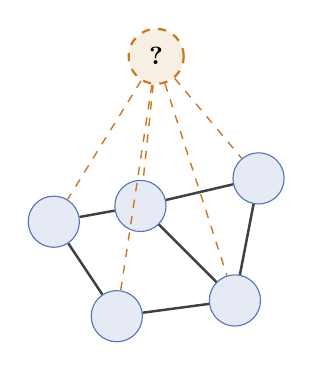
\begin{tikzpicture}[n/.style={circle,draw=costc!80,fill=costc!12,minimum size=6.5mm,inner sep=0pt,font=\small}]
  \node[n](n1) at (0,0){}; \node[n](n2) at (1.5,0.35){};
  \node[n](n3) at (1.2,-1.2){}; \node[n](n4) at (-0.3,-1.4){};
  \node[n](n5) at (-1.1,-0.2){};
  \draw[core] (n1)--(n2); \draw[core] (n2)--(n3); \draw[core] (n3)--(n4);
  \draw[core] (n4)--(n5); \draw[core] (n5)--(n1); \draw[core] (n1)--(n3);
  \node[circle,draw=newc,dashed,line width=0.8pt,fill=newc!12,minimum size=7mm,inner sep=0pt,font=\small\bfseries](N) at (0.2,1.9){?};
  \foreach \t in {n1,n2,n3,n4,n5}
    {\draw[newc,dashed,line width=0.5pt] (N)--(\t);}
\end{tikzpicture}}
\caption{Expansion: propose}
\label{sub:expand}
\end{subfigure}
\hfill
\begin{subfigure}{0.49\textwidth}\centering
\resizebox{0.95\linewidth}{!}{%
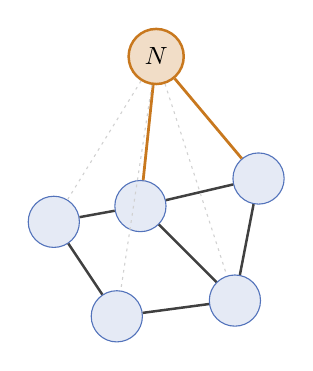
\begin{tikzpicture}[n/.style={circle,draw=costc!80,fill=costc!12,minimum size=6.5mm,inner sep=0pt,font=\small}]
  \node[n](n1) at (0,0){}; \node[n](n2) at (1.5,0.35){};
  \node[n](n3) at (1.2,-1.2){}; \node[n](n4) at (-0.3,-1.4){};
  \node[n](n5) at (-1.1,-0.2){};
  \draw[core] (n1)--(n2); \draw[core] (n2)--(n3); \draw[core] (n3)--(n4);
  \draw[core] (n4)--(n5); \draw[core] (n5)--(n1); \draw[core] (n1)--(n3);
  \node[circle,draw=newc,line width=0.9pt,fill=newc!25,minimum size=7mm,inner sep=0pt,font=\small\bfseries](N) at (0.2,1.9){$N$};
  % survivors
  \draw[newc,line width=1.0pt] (N)--(n1); \draw[newc,line width=1.0pt] (N)--(n2);
  % pruned (faint)
  \foreach \t in {n3,n4,n5}
    {\draw[black!18,dash pattern=on 1pt off 1.6pt,line width=0.4pt] (N)--(\t);}
\end{tikzpicture}}
\caption{Reduction: dispose}
\label{sub:reduce}
\end{subfigure}
\caption{Structure learning as expansion and reduction. \subref{sub:expand}~To entertain a
commitment not yet in the model, the agent proposes a new node $N$ wired tentatively to every
existing commitment by candidate edges with free priors ($\alpha_e\to 0$, amber, dashed).
\subref{sub:reduce}~Bayesian model reduction prunes the proposal in closed form, keeping only the
couplings the data support (solid) and refunding the rest by Occam (faint). Expansion costs a real
inversion because the new node may enlarge the likelihood's support; the subsequent pruning is the
cheap closed-form half. Run on a cosmology world in which the truth grows an unconceived dimension,
this move discovers that dimension only after it appears (\S\ref{sec:res-explore}).}
\label{fig:bmebmr}
\end{figure}

\subsection{Temporal structure: accumulation and forgetting}
\label{sec:temporal}

The operator of \S\ref{sec:carryover} is static. Read once from a fixed set of coupling
precisions, $\kappa=\Top\bone$ can only grow as structure learning adds edges, and nothing
lets an unreinforced dependency loosen: a paradigm with no forgetting is a ratchet. This is
both unrealistic and---as the population experiments confirm sharply
(\S\ref{sec:res-forgetting})---the degenerate limit in which lock-in is automatic
rather than earned.

Active inference carries the missing ingredient and we import it unmodified. In the
process-theoretic treatment of learning, the parameters of the generative model are not
constants but are carried by conjugate hyperparameters whose concentration accumulates with
corroborating evidence; forgetting is a multiplicative \emph{forgetting factor}
$\omega\in(0,1]$ applied to that accumulated concentration between updates
\citep{friston2017process,smith2022tutorial}. In the discrete case this acts on Dirichlet
counts; in the ARD parameterization of \S\ref{sec:structurelearning} it acts on the Gamma
hyperparameters of the edge precisions $\alpha_e$, the linear-Gaussian conjugate analogue.
Either way an edge precision is the posterior expectation of a parameter whose evidence
leaks at rate $\omega$ unless refreshed. Concretely, between updates the accumulated
information relaxes toward the prior, $\Pi\leftarrow\Pi_0+\omega(\Pi-\Pi_0)$, so a deposit
$k$ steps old carries weight $\omega^k$ (an exponential memory of $\sim 1/(1-\omega)$ steps).
The factor is not arbitrary: it is the agent's
prior on the rate of structural drift in the world, the same quantity that volatility
estimation makes learnable in the hierarchical Gaussian filter \citep{mathys2011}---one
forgets at the rate one believes the world's structure is moving. We sweep $\omega$ here
and leave its inference to the volatility machinery.

The operator inherits the time index. With $A_t$ rebuilt each round from the decayed-and-
reaccumulated precisions, $\Top_t=(I-A_t)^{-1}$, and conservatism becomes $\kappa_t=\Top_t
\bone$: a once-central node whose couplings are no longer reinforced relaxes back toward
cheapness, and the ratchet is gone. The closed forms of \S\ref{sec:bmebmr}--\ref{sec:both}
are unaffected, because $\Top_t$ is fixed \emph{within} a round; the model is a sequence of
within-round-stationary problems, and stationarity across rounds was never used.

The decisive choice is what \emph{not} to decay. In its sharpest form one applies the forgetting
factor to the coupling precisions alone and leaves the utility source $u$ intact. The asymmetry is
not a second free parameter but the mechanism: under $U=\Top_t u$ the operator relaxes while the
source persists, so a commitment can lose its structural support entirely---$\kappa_t$
drained, the couplings that justified it forgotten---yet keep its conviction. This is the
temporal face of the linear-independence of \S\ref{sec:twofields}: the static result lets
the two fields disagree about \emph{where}, forgetting lets them disagree about \emph{when},
and motivated persistence (a belief wanted-true after its reasons have leaked away) becomes
a consequence of the single inequality $\omega_\pi<1\le\omega_u$ rather than a posited bias.
In the experiments of \S\ref{sec:res-forgetting} we use the minimal, symmetric version (one
$\omega$ on all accumulated information), and find that it already turns lock-in from automatic
into a \emph{conviction threshold}; the asymmetric $\omega_\pi<\omega_u$ would make that
persistence permanent rather than threshold-gated. Decay applied instead to the \emph{gating}
precisions $\rho_k$ would relax $\gamma$ itself, turning a permanent stall into a race between
structural relaxation and conviction reinforcement; we note this as the sharper reading of lock-in.


% ======================================================================
\section{A value field: belief utility and motivated revision}
\label{sec:twofields}
% ======================================================================

The structure-learning account of Section~\ref{sec:bmebmr} makes belief change a matter of inferential
cost and evidence alone, but precision does not determine which commitments a scientist attends to or
propagates. The literature on the division of cognitive labour is explicit that attention is allocated
for reasons that are not purely epistemic: scientists distribute themselves across research programmes
by pursuing credit and reward under the priority rule, not by maximizing expected information
\citep{kitcher1990,strevens2003}, and funding priorities, disciplinary prestige, and institutional
commitment shape which questions are pursued and which results defended. A result on which a career
rests is held more tightly than its evidence warrants; a programme is sustained because it is fundable.
These are not noise on inference but a second organizing field over the same commitments---an
attentional or valence field assigning each belief an intrinsic utility independent of its precision.
The variational-cost account of belief revision \citep{hyland2025} gives this field its formal handle,
treating belief change as a motivated decision that trades the informational cost of revision against
the utility of the belief held. It is this value field, and not a refinement of the cost field, that
the present section adds.

Active inference already supplies the formal slot for it: the preference matrix $\mathbf{C}$, the
log-probabilities of the observations an agent expects and prefers to see. Read through
\citet{hyland2025}, this becomes a \emph{belief utility}---a value attached to holding a belief over
and above its accuracy, the signature of a boundedly rational agent for whom some conclusions matter
more than others. That such a utility should live on a \emph{network} rather than on a single belief
is not our invention but an established empirical posture: the Causal Attitude Network model
\citep{dalege2016} treats a belief system as a network of evaluative reactions in which connectivity
is attitude strength, which is exactly the structural reading of conviction we now formalize. The key
step is that conviction propagates through the conditional structure by the \emph{same operator} that
propagates cost---a commitment one intrinsically wants true lends value to its dependents---so the
conviction field is
\begin{equation}
U \;=\; \Top\,u,
\qquad\text{i.e.}\qquad
U_i \;=\; u_i+\!\!\sum_{w\in\desc(i)}\!\!\pi_{i\rw w}\,u_w ,
\label{eq:U}
\end{equation}
where $u$ is the vector of intrinsic utilities. The same operator $\Top$ acts on two source vectors:
the unit source $\bone$ yields conservatism (Eq.~\ref{eq:kappa}), the utility source $u$ yields
conviction (Eq.~\ref{eq:U}). This is the precise content of the two-field claim, and it renders the
\emph{decoupling} of Fig.~\ref{fig:twofields} a one-line statement: $\Top\bone$ and $\Top u$ are
linearly independent unless $u\propto\bone$, that is, unless every commitment is valued in exact
proportion to its mere presence. A commitment may be costly to revise yet value-neutral---a deeply
embedded technical posit no one has feelings about---or cheap yet cherished, a peripheral belief one
is nonetheless attached to. The misalignment of the two colorings in Fig.~\ref{fig:twofields} is
exactly this linear independence, and Section~\ref{sec:res-twofield} exhibits it on a real net.

\paragraph{The revision objective and its two cumulants.}
With conviction in hand we can write the objective the motivated agent actually minimizes, rather
than only its solution. When the utility is linear in the belief, belief revision is the minimization
of a free energy that trades the fidelity of the honest posterior against the value it can buy,
\begin{equation}
\mathcal{F}[q]\;=\;\KL{q}{p(s\mid o)}\;-\;\lambda\,\Eq{q}{U(s)},
\label{eq:revfunctional}
\end{equation}
and the Gibbs variational principle returns its minimizer in closed form, the value-tilted posterior
\begin{equation}
q_\lambda(s)\;\propto\;p(s\mid o)\,e^{\lambda U(s)} .
\label{eq:tilted}
\end{equation}
Here $\lambda$ is the tilt---a single temperature governing how far value is permitted to bend the
evidence, an object \emph{entirely distinct} from the structural conservatism $\kappa_i$ of
Eq.~\eqref{eq:kappa} despite the family resemblance of the two costs; conservatism is a property of a
node's position in the graph, the tilt a scalar on the whole ledger, and conflating them would
wrongly couple the two fields we have just shown to be independent. The normalizer of
Eq.~\eqref{eq:tilted} is a cumulant-generating function,
\begin{equation}
Z(\lambda)\;=\;\log\,\Eq{p(s\mid o)}{e^{\lambda U(s)}},
\label{eq:cgf}
\end{equation}
and this is what makes the two faces of motivated cognition one object rather than two bolted
together. The additive bias that re-centres where the agent lands is the \emph{mean} of the tilted
ledger, $\Eq{q_\lambda}{U}=Z'(\lambda)$; the multiplicative bias that sets how strongly any channel
can move the agent is its \emph{variance}, the susceptibility $\Var{q_\lambda}{U}=Z''(\lambda)$. The
two biases are the first two cumulants of one tilted ledger. A disconfirming channel held near zero
sensory precision $\rho_k$ contributes nothing to that variance, so no tilt along it can move the
evidence at all: the agent runs ordinary structure learning, but reads its ledger at a displaced mean
and with a curvature its own precision field has flattened along the disconfirming directions.

\paragraph{From gating to a population quantity.}
It is this gating that becomes, in Section~\ref{sec:model}, the order parameter $\gamma$, and we
define it here so that it is built rather than imported. Let the disconfirming sensory channels of a
paradigm be those whose evidence would license a core revision, with total precision
$\sum_{k\in\mathrm{dis}}\rho_k$. The conviction field can drive a subset of these toward
$\rho_k\approx 0$---curvature flattened where it would hurt most. Define
\begin{equation}
\gamma\;=\;\frac{\sum_{k\in\mathrm{dis}}\rho_k\,\mathbb{1}[\,\rho_k\ \text{gated by the core}\,]}
{\sum_{k\in\mathrm{dis}}\rho_k},
\label{eq:gamma}
\end{equation}
the fraction of the disconfirming sensory precision the core's conviction field has silenced. Lock-in
(Section~\ref{sec:model}) follows from Eq.~\eqref{eq:gamma} through the susceptibility $Z''(\lambda)$:
when $\gamma$ is large, the susceptibility along the disconfirming directions is driven to zero, and a
value tilt cannot be displaced by evidence those directions no longer transmit.

\begin{figure}[t]
\centering
\begin{subfigure}{0.49\textwidth}\centering
\resizebox{\linewidth}{!}{%
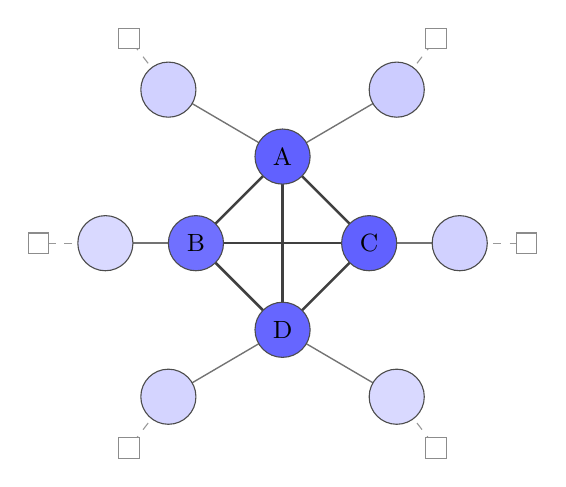
\begin{tikzpicture}
  \Positions \Edges
  \node[bel,fill=blue!62!white] at (A){A};
  \node[bel,fill=blue!56!white] at (B){B};
  \node[bel,fill=blue!62!white] at (C){C};
  \node[bel,fill=blue!60!white] at (D){D};
  \node[bel,fill=blue!18!white] at (b1){};
  \node[bel,fill=blue!20!white] at (b2){};
  \node[bel,fill=blue!15!white] at (b3){};
  \node[bel,fill=blue!18!white] at (b4){};
  \node[bel,fill=blue!17!white] at (b5){};
  \node[bel,fill=blue!15!white] at (b6){};
\end{tikzpicture}}
\par\vspace{4pt}
\resizebox{0.8\linewidth}{!}{%
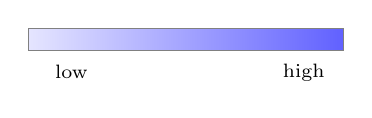
\begin{tikzpicture}
  \shade[left color=blue!10!white,right color=blue!62!white] (0,0) rectangle (4,0.28);
  \draw[black!50,line width=0.3pt] (0,0) rectangle (4,0.28);
  \node[font=\scriptsize] at (0.55,-0.28){low}; \node[font=\scriptsize] at (3.5,-0.28){high};
\end{tikzpicture}}
\caption{Revision cost $\kappa_i$ (conservatism)}
\label{sub:cost}
\end{subfigure}
\hfill
\begin{subfigure}{0.49\textwidth}\centering
\resizebox{\linewidth}{!}{%
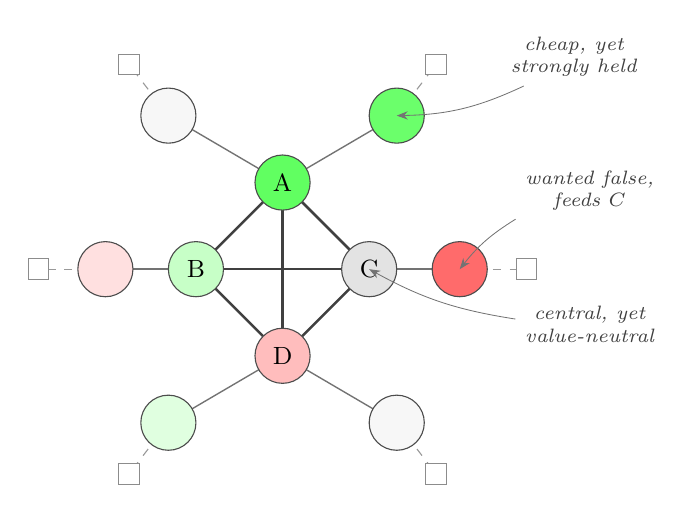
\begin{tikzpicture}
  \Positions \Edges
  \node[bel,fill=green!62!white] at (A){A};
  \node[bel,fill=green!22!white] at (B){B};
  \node[bel,fill=gray!22!white]  at (C){C};
  \node[bel,fill=red!26!white]   at (D){D};
  \node[bel,fill=gray!6!white]   at (b1){};
  \node[bel,fill=green!58!white] at (b2){};
  \node[bel,fill=red!12!white]   at (b3){};
  \node[bel,fill=red!58!white]   at (b4){};
  \node[bel,fill=green!12!white] at (b5){};
  \node[bel,fill=gray!6!white]   at (b6){};
  \node[anno] (an2) at (3.7,2.7){cheap, yet\\strongly held};
  \draw[annoarrow] (an2) to[bend left=12] (b2);
  \node[anno] (anC) at (3.9,-0.7){central, yet\\value-neutral};
  \draw[annoarrow] (anC) to[bend left=10] (C);
  \node[anno] (an4) at (3.9,1.0){wanted false,\\feeds $C$};
  \draw[annoarrow] (an4) to[bend right=10] (b4);
\end{tikzpicture}}
\par\vspace{4pt}
\resizebox{0.95\linewidth}{!}{%
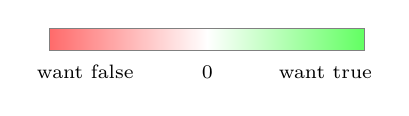
\begin{tikzpicture}
  \shade[left color=red!58!white,right color=white] (0,0) rectangle (2,0.28);
  \shade[left color=white,right color=green!62!white] (2,0) rectangle (4,0.28);
  \draw[black!50,line width=0.3pt] (0,0) rectangle (4,0.28);
  \node[font=\scriptsize] at (0.45,-0.28){want false}; \node[font=\scriptsize] at (2,-0.28){0};
  \node[font=\scriptsize] at (3.5,-0.28){want true};
\end{tikzpicture}}
\caption{Intrinsic utility $u_i$ (conviction)}
\label{sub:util}
\end{subfigure}
\caption{Two fields on one paradigm (schematic). Both panels carry the \emph{same} network---a densely
coupled core $\{A,B,C,D\}$ and a sparse belt $\{b_1,\dots,b_6\}$ in contact with observation.
\subref{sub:cost}~Revision cost is the carry-over of mind-change, $\kappa=\Top\bone$
(Eq.~\ref{eq:kappa}): a node's cost is the precision-weighted mass of its descendants, a clean radial
gradient monotone in centrality. \subref{sub:util}~Intrinsic utility is signed---beliefs one wants
true (green), wants false (red), or is neutral toward (white)---and the conviction field
$U=\Top u$ does not align with $\kappa$: $C$ is central yet value-neutral; $b_2$ is cheap yet strongly
held; $b_4$, which feeds $C$, is a conclusion the community wants false. The two fields are
$\Top\bone$ and $\Top u$, the same operator on two sources, and they are independent vectors.
Fig.~\ref{fig:res-twofield} shows this decoupling computed on a real dark-energy net.}
\label{fig:twofields}
\end{figure}

% ======================================================================
\section{Coupling of the two fields under model expansion}
\label{sec:both}
% ======================================================================

The two fields are coupled by the expansion operation, and with $\Top$ defined the coupling follows
directly. When the agent expands its model---proposing a new commitment $N$ wired by candidate
conditionals to a set of existing nodes---the joint gains an explicit factor,
\begin{equation}
p(x,x_N\mid G')\;\propto\;p(x\mid G)\!\!\prod_{(N\leftrightarrow v)}\!\!\psi_{Nv}(x_v,x_N)^{\pi_{Nv}},
\label{eq:expand}
\end{equation}
with the candidate edges entered at free prior precision ($\alpha_e\to 0$) so that reduction can
carve them back. In operator terms, adding $N$ appends a row and a column to $A$---and therefore to
$\Top$---and appends one entry to \emph{each} of the two source vectors, the unit source $\bone$ and
the utility source $u$. The two consequences are then immediate. Every node $N$ touches gains the new
coupling precision it must now also propagate,
\begin{equation}
\Delta\kappa_v \;=\; \pi_{Nv},
\label{eq:dkappa}
\end{equation}
while the conviction field gains, at $N$ and along its new edges,
\begin{equation}
\Delta U \;=\; u_N+\!\!\sum_{w\in\desc(N)}\!\!\pi_{N\rw w}\,u_w .
\label{eq:dU}
\end{equation}
A single expansion thus writes the new commitment into both the cost geometry and the value geometry
(Fig.~\ref{fig:both}). This is the precise content of motivated structure learning: an agent
contemplating a node that would, once wired in, lend value to a cherished core---or force the revision
of one---registers that prospect in \emph{both} fields, as a carry-over cost it must pay and as a value
change it may welcome or resist, and scores the keep-or-prune decision against the value-tilted ledger
of Eqs.~\eqref{eq:revfunctional}--\eqref{eq:tilted}. The same proposal can therefore be evidence-favoured
and value-rejected, or the reverse.

\begin{figure}[t]
\centering
\begin{subfigure}{0.49\textwidth}\centering
\resizebox{0.95\linewidth}{!}{%
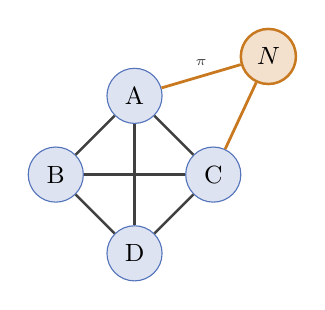
\begin{tikzpicture}[n/.style={circle,draw=costc!80,fill=costc!16,minimum size=7mm,inner sep=0pt,font=\small}]
  \node[n](A) at (0,1){A}; \node[n](B) at (-1,0){B};
  \node[n](C) at (1,0){C}; \node[n](D) at (0,-1){D};
  \draw[core] (A)--(B); \draw[core] (A)--(C); \draw[core] (A)--(D);
  \draw[core] (B)--(C); \draw[core] (B)--(D); \draw[core] (C)--(D);
  \node[circle,draw=newc,line width=0.9pt,fill=newc!22,minimum size=7mm,inner sep=0pt,font=\small\bfseries](N) at (1.7,1.5){$N$};
  \draw[newc,line width=1.0pt] (N)--(A) node[midway,above,font=\tiny,text=black!70]{$\pi$};
  \draw[newc,line width=1.0pt] (N)--(C);
\end{tikzpicture}}
\caption{enters the belief network (coupling $\pi$, $\Delta\kappa_v=\pi_{Nv}$)}
\label{sub:bel}
\end{subfigure}
\hfill
\begin{subfigure}{0.49\textwidth}\centering
\resizebox{0.95\linewidth}{!}{%
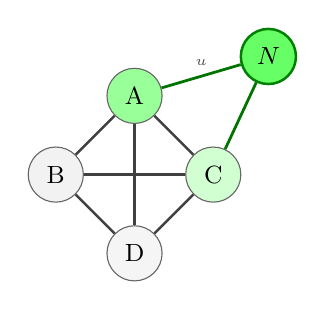
\begin{tikzpicture}[n/.style={circle,draw=black!60,minimum size=7mm,inner sep=0pt,font=\small}]
  \node[n,fill=green!40!white](A) at (0,1){A}; \node[n,fill=gray!10!white](B) at (-1,0){B};
  \node[n,fill=green!18!white](C) at (1,0){C}; \node[n,fill=gray!8!white](D) at (0,-1){D};
  \draw[core] (A)--(B); \draw[core] (A)--(C); \draw[core] (A)--(D);
  \draw[core] (B)--(C); \draw[core] (B)--(D); \draw[core] (C)--(D);
  \node[circle,draw=green!50!black,line width=0.9pt,fill=green!60!white,minimum size=7mm,inner sep=0pt,font=\small\bfseries](N) at (1.7,1.5){$N$};
  \draw[green!45!black,line width=1.0pt] (N)--(A) node[midway,above,font=\tiny,text=black!70]{$u$};
  \draw[green!45!black,line width=1.0pt] (N)--(C);
\end{tikzpicture}}
\caption{enters the utility network (propagated value, $\Delta U$)}
\label{sub:val}
\end{subfigure}
\caption{One expansion, two fields. Adding a commitment $N$ with new conditionals appends a row and a
column to the operator $\Top$ and an entry to each source vector: into the belief network, where each
new edge carries a coupling precision $\pi$ and so adds to carry-over cost by
Eq.~\eqref{eq:dkappa} (a), and into the utility network, where $N$'s value propagates along the same
new edges by Eq.~\eqref{eq:dU} and tints the commitments it reaches (b). The keep-or-prune decision is
scored against the value-tilted ledger, so a proposal can be evidence-favoured yet value-rejected, or
the reverse.}
\label{fig:both}
\end{figure}

% ======================================================================
\section{A population model of collective structure learning}
\label{sec:model}
% ======================================================================

The full model can now be stated. A population of $N$ agents inhabits a shared but hidden world. Each
agent carries its own paradigm network over that world---its own structure, its own coupling
precisions, its own conviction field $U=\Top u$, and a conservatism profile $\kappa=\Top\bone$ read
from its connectivity by Eq.~\eqref{eq:kappa}. Each agent performs structure learning: it samples the
world through its belt under expected free energy, prunes by Bayesian model reduction the couplings
the data fail to support, and occasionally expands by proposing a new node, writing it into both
fields. The agents are coupled. A peer transmits not a scalar opinion but a \emph{candidate structural
revision}---a proposed node or edge, together with the precisions it would carry. The receiver treats
that transmission as an external source it may trust or distrust, importing the revision weighted by a
trust-channel precision $\pi_s$; that is, it performs ordinary active-inference updating on the peer's
proposal exactly as it would on a sensory channel, with $\pi_s$ playing for the social edge the role
$\rho_k$ plays for the senses. The distinction the scalar models could only assert now follows from
the representation: a \emph{bubble} is a missing channel, which exposure dissolves, whereas an
\emph{echo chamber} is a channel present but held at $\pi_s\approx 0$, which exposure only reinforces
\citep{nguyen2018}. A third hand acts on this same $\pi_s$, external to both the agent and her
peers---the \emph{curator}: the recommendation, ranking, and visibility filters of research practice
that set, from outside, which revisions reach an agent at all.

The model is built to test whether paradigm learning emerges when a population learns structure
together, sharing candidate revisions across a trust network. Because the prediction of interest is
organized by conservatism---belt-first, core-last---we resolve the order parameter \emph{by}
conservatism rather than collapsing it to a single scalar, which would discard the structural
resolution the model is intended to expose. Fix a node alignment between agent $a$'s network and the
rival target structure $G^\ast$, and let $\mathrm{align}^a_i(t)\in[0,1]$ be the fraction of node $i$'s
incident coupling mass whose couplings agree with $G^\ast$ under that alignment---a structural
agreement, not an indicator that a single edge ``became'' a rival edge. Splitting the nodes by
conservatism into a belt and a core, $S_{\mathrm{belt}}=\{i:\kappa_i<\tau\}$ and
$S_{\mathrm{core}}=\{i:\kappa_i\ge\tau\}$, define the stratified order parameter
\begin{equation}
m_S(t)\;=\;\frac{1}{N}\sum_{a=1}^{N}
\frac{\sum_{i\in S}\mu_i\,\mathrm{align}^a_i(t)}{\sum_{i\in S}\mu_i},
\qquad S\in\{\mathrm{belt},\mathrm{core}\},
\label{eq:order}
\end{equation}
with $\mu_i$ node $i$'s incident coupling mass. A scalar account, with one variable to flip, predicts
a single sharp cascade. The structural account predicts a separation between the two curves:
$m_{\mathrm{belt}}(t)$ rises first as the cheap periphery reorganizes, and $m_{\mathrm{core}}(t)$
follows only once enough evidence has accumulated to pay the core's carry-over cost
(Fig.~\ref{fig:phase}). The gap between the belt and core curves is the staircase. Whether this
staircase survives in a runnable linear-Gaussian implementation is one of the questions
Section~\ref{sec:results} settles---and the honest answer (\S\ref{sec:res-staircase}) is that it does
not, for a reason worth stating precisely.

A third regime is produced by the value field, and its mechanism must be distinguished from that of
conservatism. Conservatism alone cannot produce a stall: a high-$\kappa$ core is merely \emph{slow}---the
belt--core gap widens and the delay lengthens---but the disconfirming evidence still arrives,
accumulates, and the core eventually pays its cost and moves ($m_{\mathrm{core}}\to$ high,
Fig.~\ref{fig:phase}, teal). Permanent stall is a $\gamma$-phenomenon. When $\gamma$
(Eq.~\ref{eq:gamma}) is large the channels carrying the rival's characteristic anomaly are held near
zero precision, their susceptibility $Z''(\lambda)$ along the disconfirming directions flattened to
nothing, so the cheap belt revisions still happen but the evidence that would license the core
revision never arrives, and $m_{\mathrm{core}}(t)$ rises a little and then stalls below unity despite
physically present disconfirming data (Fig.~\ref{fig:phase}, violet). Centrality sets how slowly the
core moves; conviction sets whether it moves at all. The crossover in $\gamma$ is a phase boundary,
and the stalled core curve---a community that has seen the anomaly and not moved---is the model's
sharpest prediction.

\begin{figure}[t]
\centering
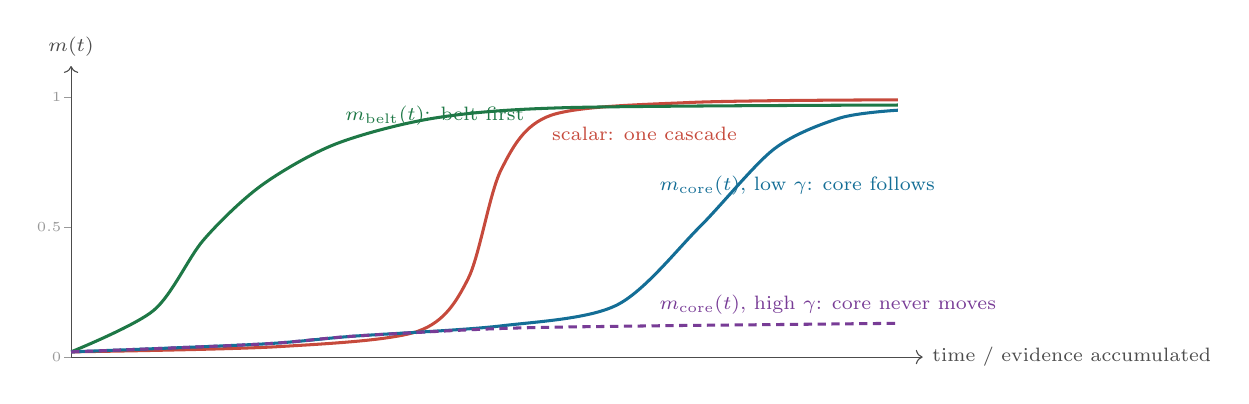
\begin{tikzpicture}[xscale=1.05,yscale=3.3]
  \draw[->,black!70] (0,0) -- (10.3,0) node[right,font=\scriptsize]{time / evidence accumulated};
  \draw[->,black!70] (0,0) -- (0,1.12) node[above,font=\scriptsize]{$m(t)$};
  \foreach \y in {0,0.5,1} \draw[black!40] (-0.08,\y)--(0,\y) node[left,font=\tiny]{\y};
  % scalar model: single sharp cascade
  \draw[scalarc,line width=1.1pt,smooth] plot coordinates
    {(0,0.02)(2.5,0.04)(4.2,0.10)(4.8,0.30)(5.2,0.72)(5.8,0.93)(7.5,0.98)(10,0.99)};
  % belt curve: rises early, saturates high (shared across regimes)
  \draw[gradc,line width=1.1pt,smooth] plot coordinates
    {(0,0.02)(1.0,0.18)(1.6,0.45)(2.3,0.66)(3.2,0.82)(4.4,0.92)(6,0.96)(10,0.97)};
  % core curve, low gamma: rises late, reaches high
  \draw[corec,line width=1.1pt,smooth] plot coordinates
    {(0,0.02)(2.3,0.05)(3.4,0.08)(5.2,0.12)(6.6,0.20)(7.6,0.50)(8.5,0.80)(9.3,0.92)(10,0.95)};
  % core curve, high gamma: stalls
  \draw[lockc,line width=1.1pt,dash pattern=on 3pt off 2pt,smooth] plot coordinates
    {(0,0.02)(2.3,0.05)(3.4,0.08)(5.2,0.11)(7,0.12)(8.5,0.125)(10,0.13)};
  \node[scalarc,font=\scriptsize,anchor=west] at (5.7,0.86){scalar: one cascade};
  \node[gradc,font=\scriptsize,anchor=west] at (3.2,0.93){$m_{\mathrm{belt}}(t)$: belt first};
  \node[corec,font=\scriptsize,anchor=west] at (7.0,0.66){$m_{\mathrm{core}}(t)$, low $\gamma$: core follows};
  \node[lockc,font=\scriptsize,anchor=west] at (7.0,0.20){$m_{\mathrm{core}}(t)$, high $\gamma$: core never moves};
\end{tikzpicture}
\caption{The \emph{predicted} central contrast (schematic). A scalar order parameter (red) has one
inflection; the conservatism-stratified order parameter of Eq.~\eqref{eq:order} is predicted to
separate into a belt-first / core-last staircase, with a $\gamma$-gated stall at high conviction.
Section~\ref{sec:results} reports what the implemented model actually does: the population signatures
(re-tracking, lock-in, motivated persistence) are recovered, but the staircase by conservatism washes
out for the reason given in \S\ref{sec:res-staircase}.}
\label{fig:phase}
\end{figure}

% ======================================================================
\section{Results: running the model}
\label{sec:results}
% ======================================================================

We implemented the model as a linear-Gaussian Bayesian network with the closed forms of
\S\ref{sec:bmebmr}--\ref{sec:both} and ran it in two settings. The first is a single-agent
\emph{dark-energy} paradigm net---general relativity (GR) at the root; the density parameters
$\Omega_m$ and the cosmological constant $\Lambda$ as dials; the Friedmann expansion, distance
modulus $\mu(z)$ and a Type-Ia supernova (SN) reading as a descending chain; light-bending, the
perihelion precession, gravitational redshift, CMB and BBN as GR's other branches; and a
modified-gravity (MOND) prediction the community wants false---which makes the two fields and the
Schur residue concrete. The second is a population of $N=150$ agents in three communities tracking a
\emph{changing-cosmology} world whose true theory shifts at $t=60$ and $t=120$ through dark-matter,
modified-gravity and scale-variant regimes. All code is seeded and ships its own null/positive
controls. We report what the model does, including---\S\ref{sec:res-caveats}---where it departs from
the schematic prediction of Fig.~\ref{fig:phase}.

\subsection{The two fields are realised, and decoupled}
\label{sec:res-twofield}

Computing $\kappa=\Top\bone$ and $U=\Top u$ on the dark-energy net (Fig.~\ref{fig:res-twofield})
makes the two-field claim of \S\ref{sec:twofields} concrete. Conservatism is steepest at GR
($\kappa_{\mathrm{GR}}=10.5$, the maximum) and shallow at the cosmological constant
($\kappa_\Lambda=2.85$, a ratio of $3.7$): GR carries every predicted observable below it, $\Lambda$
only the distance--redshift branch. This is Lakatos's belt-protects-core falling straight out of the
operator---when the 1998 anomaly arrives at the bottom, the cheap move is to turn the dial with the
smallest descendant set ($\Lambda$), not the ancestor with the largest (GR). The conviction field
$U=\Top u$, with the community valuing the accelerating-universe supernova reading ($u_{\mathrm{SN}}=+1$),
the $\Lambda$ commitment ($+0.6$) and wanting MOND false ($-0.8$), \emph{inverts} that order:
$U_\Lambda=1.19$ (the most cherished) exceeds $U_{\mathrm{GR}}=0.45$ while $\kappa_\Lambda<\kappa_{\mathrm{GR}}$.
The two fields are linearly independent (Pearson $r(\kappa,U)=0.25$): $\Lambda$ is \emph{cheap yet
cherished}, GR \emph{central yet comparatively value-neutral}, the GR machinery
(light-bending, perihelion, clocks, CMB, BBN) central yet value-neutral ($U\approx 0$), and MOND the
conclusion the community wants false ($U<0$)---exactly the three annotated cases of
Fig.~\ref{fig:twofields}, now read off a real net rather than drawn by hand.

\begin{figure}[t]
\centering
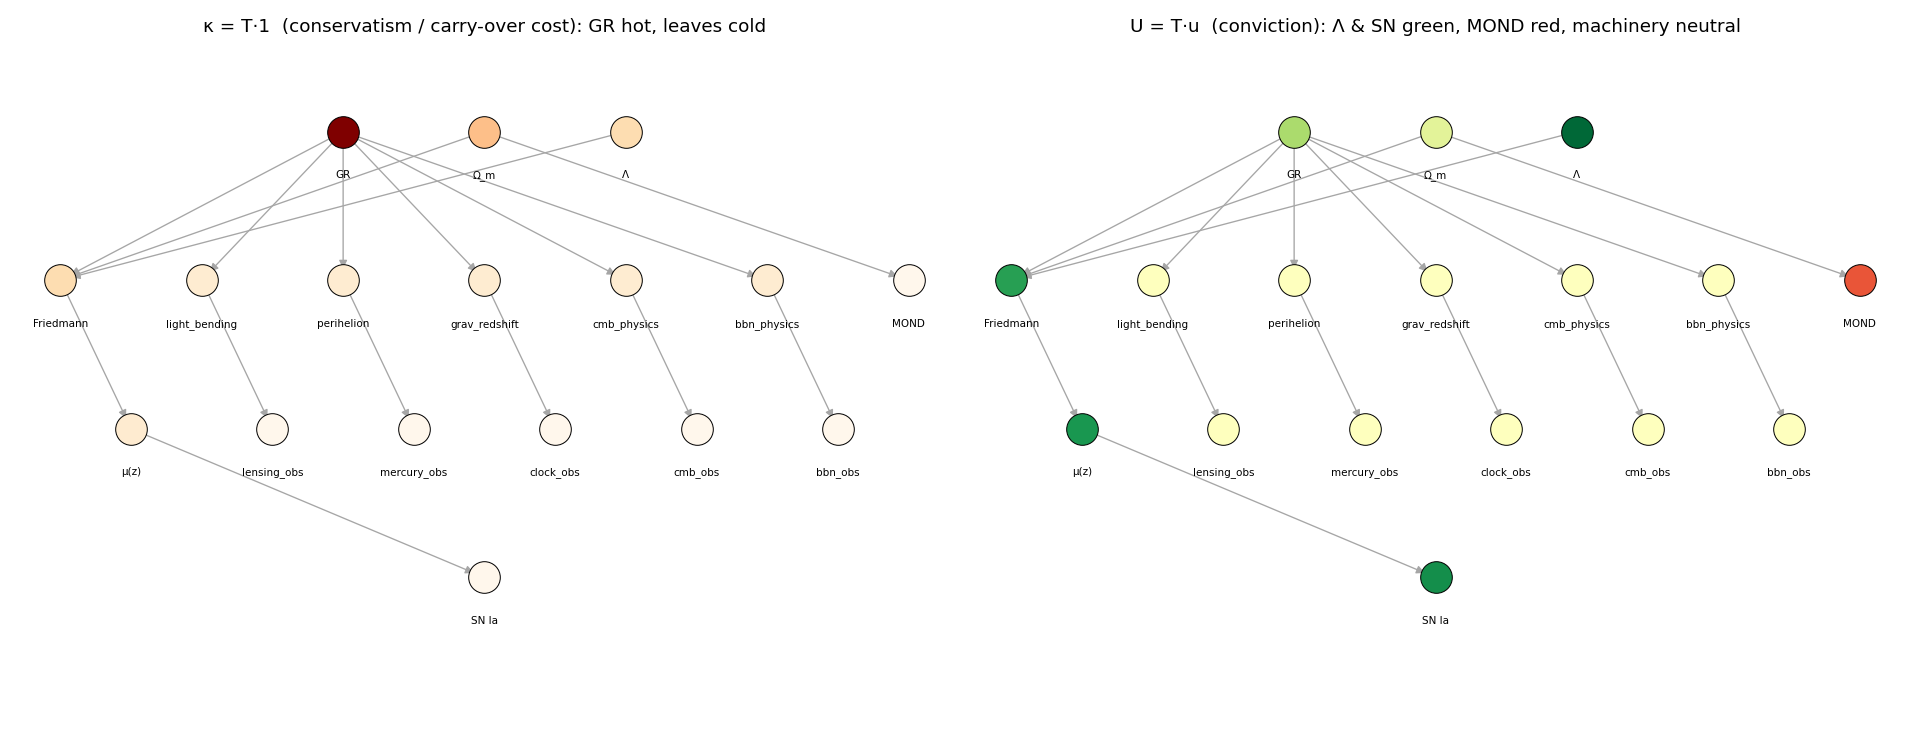
\includegraphics[width=\linewidth]{fig_two_fields_dag.png}
\caption{The two fields, computed on the dark-energy paradigm net. \emph{Left:} conservatism
$\kappa=\Top\bone$ (Eq.~\ref{eq:kappa})---GR is hot ($\kappa=10.5$), the observation leaves cold;
the directed arrows make ``everything hangs below GR'' visible. \emph{Right:} conviction $U=\Top u$
(Eq.~\ref{eq:U}) on the same graph---$\Lambda$ and the supernova reading green (cherished), MOND red
(wanted false), GR's other machinery value-neutral. The decoupling is the realisation of
Fig.~\ref{fig:twofields}: the value order inverts the cost order ($U_\Lambda>U_{\mathrm{GR}}$ while
$\kappa_\Lambda<\kappa_{\mathrm{GR}}$; $r(\kappa,U)=0.25$).}
\label{fig:res-twofield}
\end{figure}

The Schur residue of Eq.~\eqref{eq:schur} is equally concrete. A priori $\Omega_m$ and $\Lambda$ are
independent (correlation $0.00$, a round cloud). Conditioning on the shared supernova
observation---clamping the descendant both dials feed---manufactures an off-diagonal coupling
between them where the joint had a zero: the cloud collapses onto the tilted ``banana''
(Fig.~\ref{fig:res-schur}), with correlation rising to $+0.50$. This is the
$\Omega_m$--$\Lambda$ degeneracy direction every dark-energy contour plot draws, here recovered as
the Schur complement the carry-over cost is built from---incommensurability and the contour-plot
banana the same object, read in two directions.

\begin{figure}[t]
\centering
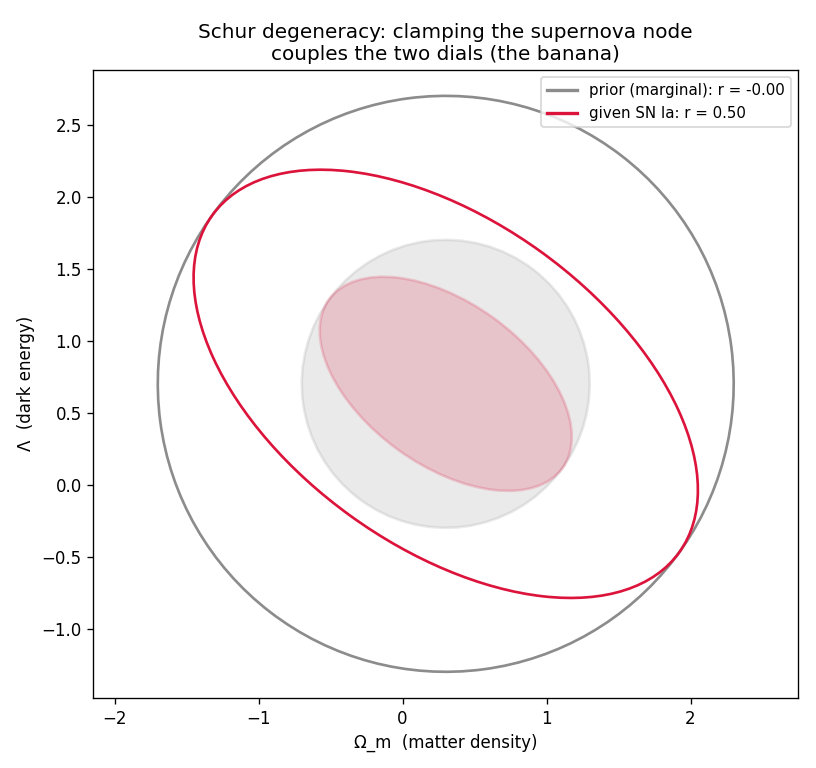
\includegraphics[width=0.52\linewidth]{fig_schur_banana.png}
\caption{The Schur degeneracy (Eq.~\ref{eq:schur}), computed. The two dials are uncorrelated a priori
(grey, $r=0.00$); conditioning on their shared supernova descendant induces the off-diagonal coupling
(crimson, $r=+0.50$)---the $\Omega_m$--$\Lambda$ ``banana''. Marginalizing a shared latent hub and
conditioning on a shared observation are the two readings of one complement.}
\label{fig:res-schur}
\end{figure}

\subsection{Lock-in requires conviction \emph{and} disconnection}
\label{sec:res-lockin}

In the population, two diversity levers are available: \emph{disconnection} (dropping the
cross-community trust density, $\pi_s\to0$, so $\lambda_2\to0$) and \emph{conviction} (the
per-community value tilt $h\leftarrow h+\lambda U$ toward a home theory). Running all four cells of
the $2\times2$ (Fig.~\ref{fig:res-tracking}) shows the levers fail \emph{differently}, and that a
durable, fragmented lock-in needs both. With neither lever, or with disconnection alone, or with
conviction alone, all three communities re-track to a single theory by the end of the run (one
distinct end-theory). Conviction alone is washed out by precision fusion---the recurring ``no-pool''
degeneracy in which naive posterior pooling erases heterogeneity. Only with \emph{both} levers do the
communities end on three different theories: the entrenched bloc, conviction-tilted to the old
incumbent \emph{and} shielded by disconnection from the evidence that would move it, stays on the
superseded theory for the whole run, while the others settle on their homes. The residual structural
disagreement (Fig.~\ref{fig:res-tracking}, right) stays high ($\approx3.3$) exactly in the
disconnected cells and collapses to $\approx0.01$ in the connected ones---the fragmented-field
signature of lock-in. This sharpens the prediction of \S\ref{sec:model}: disconnection
\emph{preserves} structural diversity; conviction \emph{converts} it into a persistent
theory-divergence, but only when disconnection protects it from fusion.

\begin{figure}[t]
\centering
\begin{subfigure}{0.62\textwidth}\centering
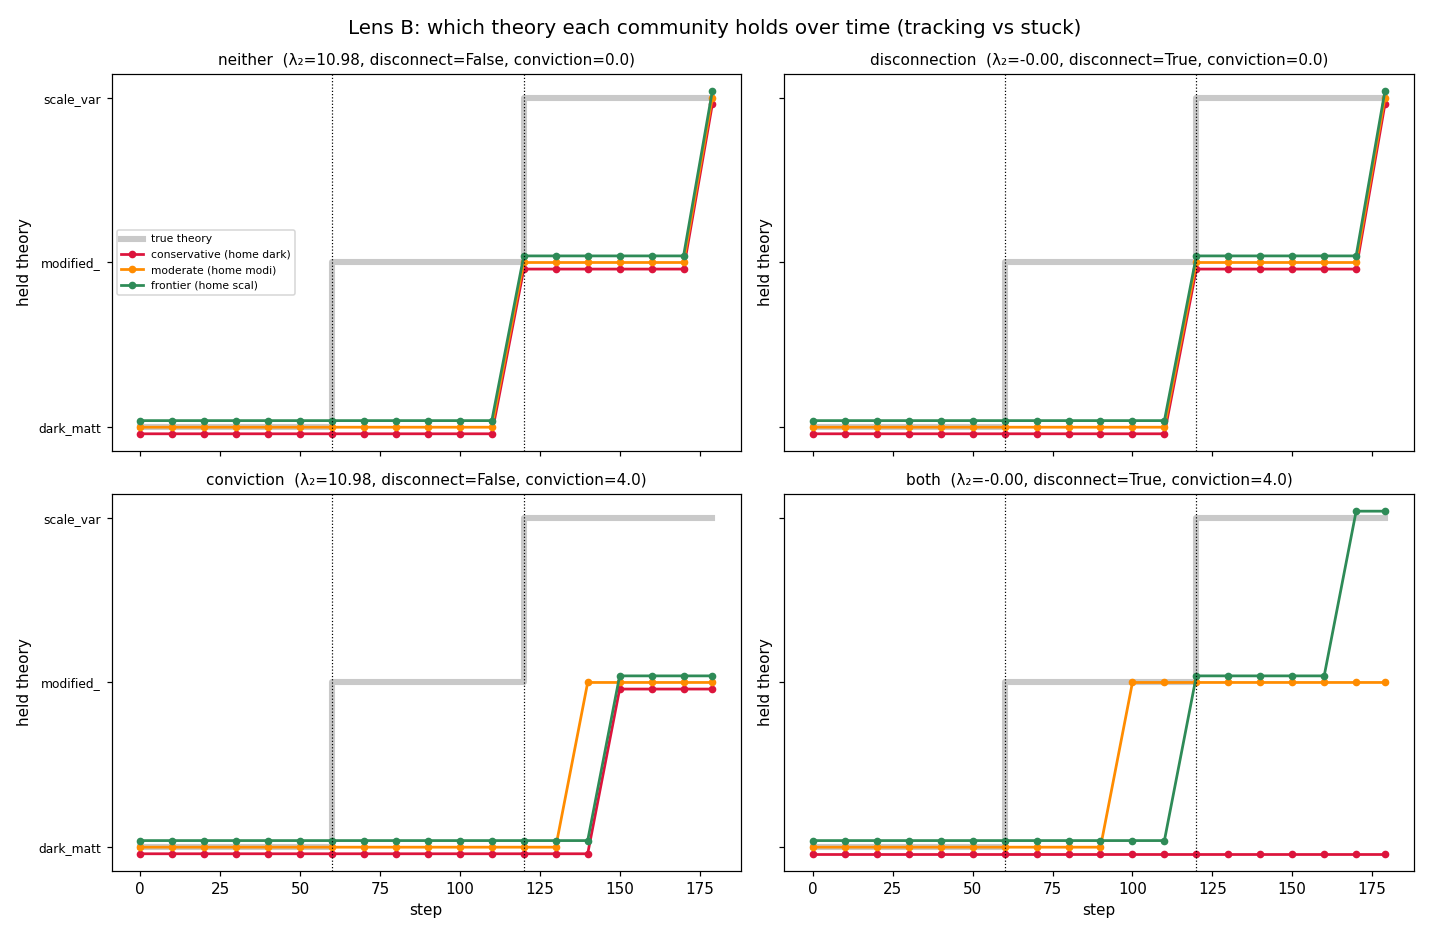
\includegraphics[width=\linewidth]{fig_tracking_2x2.png}\caption{which theory each community holds}
\label{sub:track}
\end{subfigure}\hfill
\begin{subfigure}{0.36\textwidth}\centering
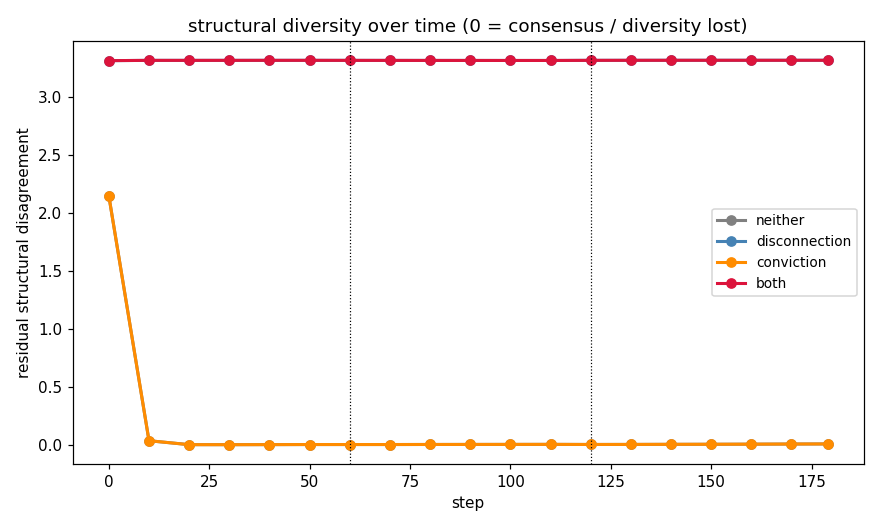
\includegraphics[width=\linewidth]{fig_diversity.png}\caption{structural diversity}
\label{sub:div}
\end{subfigure}
\caption{Population tracking of a world that changes theory three times. \subref{sub:track}~Each
community's nearest candidate theory over time; the grey staircase is the truth. Only the
\emph{both}-lever cell (disconnected + conviction) ends on three distinct theories with the
entrenched bloc stuck on the old one; the other three cells re-track to one theory.
\subref{sub:div}~Residual structural disagreement stays high in the disconnected cells (preserved
diversity / fragmented field) and collapses to consensus in the connected ones.}
\label{fig:res-tracking}
\end{figure}

\subsection{Forgetting breaks the accumulation wall, and makes lock-in earned}
\label{sec:res-forgetting}

The four cells above were run with pure accumulation ($\omega=1$), and they expose the ratchet of
\S\ref{sec:temporal} in its starkest form: a connected, lever-free population locks onto the
\emph{first} theory and never catches the moving truth---early evidence is simply too heavy by the
later epochs (Fig.~\ref{fig:res-forgetting}, the $\omega=1$ curve flat at zero after the first
shift). Switching on the forgetting factor breaks the wall cleanly: at $\omega=0.88$ the lever-free
population re-tracks each successive theory (fraction on the current true theory rising from $0.00$ to
$0.92$ in the later epochs), because a deposit decays at rate $\omega$ and the current epoch can
outweigh the stale one. The cost is confidence---steady-state precision falls from $\sim 1.1\times
10^{4}$ at $\omega=1$ to $\sim 5\times10^{2}$ at $\omega=0.88$---so there is a sweet spot around
$\omega\in[0.88,0.93]$ that re-tracks while staying confident.

\begin{figure}[t]
\centering
\begin{subfigure}{0.66\textwidth}\centering
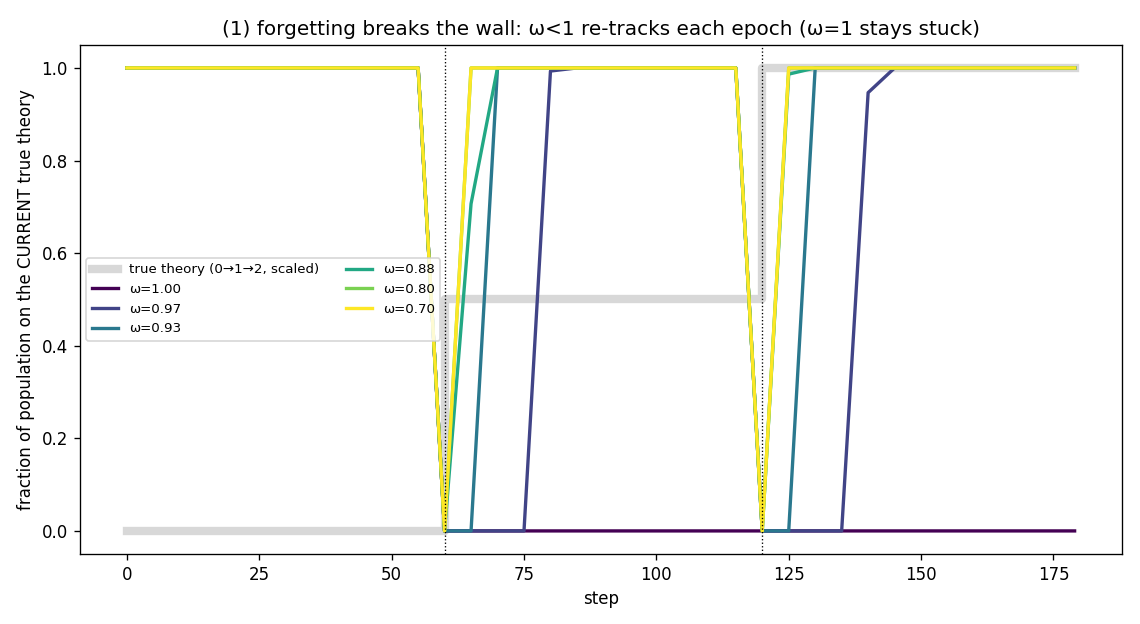
\includegraphics[width=\linewidth]{fig_wall_break.png}\caption{forgetting breaks the wall}
\label{sub:wall}
\end{subfigure}\hfill
\begin{subfigure}{0.32\textwidth}\centering
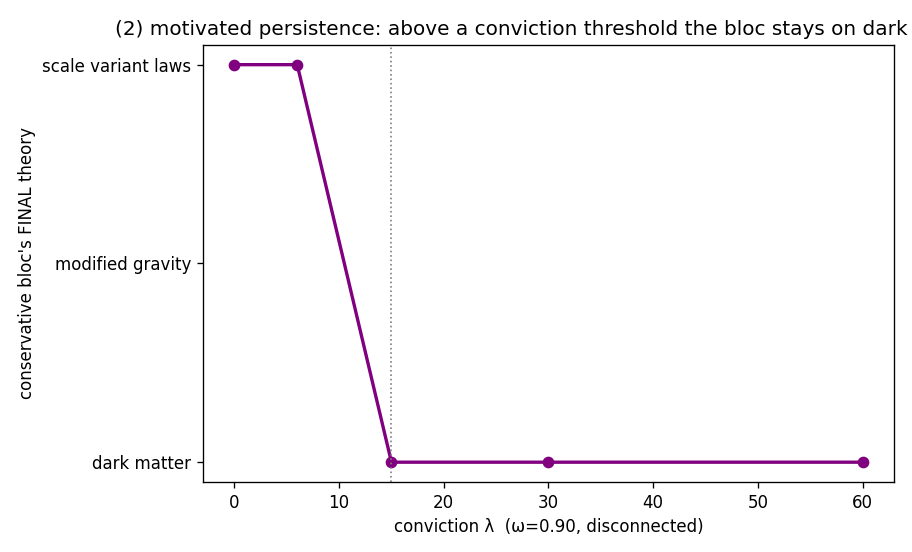
\includegraphics[width=\linewidth]{fig_motivated_persistence.png}\caption{lock-in is earned}
\label{sub:persist}
\end{subfigure}
\caption{Forgetting (precision relaxation), in the lever-free population. \subref{sub:wall}~With
$\omega=1$ the population is stuck on the first theory; with $\omega<1$ it re-tracks each epoch
(fraction on the current true theory), faster forgetting recovering sooner. \subref{sub:persist}~At
$\omega=0.90$ with disconnection, the committed bloc re-tracks for small conviction but stays on its
home theory above a conviction threshold ($\lambda\gtrsim15$): lock-in is now \emph{earned}, not
automatic---motivated persistence.}
\label{fig:res-forgetting}
\end{figure}

Forgetting also changes the character of conviction, and this is the subtler finding. Without
forgetting the value tilt accumulates without bound (it is re-applied every step and never decays),
so \emph{any} positive conviction eventually dominates the evidence---lock-in is automatic, a
degenerate consequence of the ratchet. With forgetting the tilt saturates at $\lambda U/(1-\omega)$
and competes with the (also-saturated) per-step evidence, so it holds only above a threshold. Sweeping
conviction at $\omega=0.90$ (Fig.~\ref{fig:res-forgetting}, right), the entrenched bloc re-tracks for
$\lambda\le 6$ and stays locked on its home theory for $\lambda\ge 15$. This is exactly the motivated
persistence of \S\ref{sec:temporal}---a belief held after its evidence has leaked away---turned from a
posited bias into a threshold one must clear. (We use a single symmetric $\omega$; the asymmetric
$\omega_\pi<1\le\omega_u$ of \S\ref{sec:temporal} would push the threshold to zero and make the
persistence permanent.)

\subsection{Exploration is a rate; expansion discovers the unconceived}
\label{sec:res-explore}

The exploration the network-epistemology models post as an $\epsilon$ appears here as the \emph{rate}
of a Poisson process governing when an agent proposes a structural edit. Letting the discovery of a
new node arrive at rate $\lambda$, the discovery \emph{time} becomes a waiting time rather than a
fixed instant (Fig.~\ref{fig:res-explore}, left): the mean delay between a cause appearing and the
agent finding it tracks $\approx1/\lambda$, falling from $23$ steps at $\lambda=0.02$ (where $28\%$ of
runs never discover the cause within the horizon) to $4$ steps at $\lambda=1.0$. This is the minimal,
content-free generator the paper commits to---it fixes the rate and leaves the proposal's content to
the evidence---and it makes ``too little exploration'' a precise statement: below a rate, the
community fails to find what it lacks in time.

What it lacks can be a dimension its menu does not contain. We ran an agent whose six-node cosmology
menu has no slot for $\Lambda$ against a world in which, after $t=120$, an unconceived dark-energy
cause switches on and couples commitments the menu holds independent. The cause cannot be represented
as one of the menu's nodes, so its footprint surfaces as a coherent floor in the agent's prediction
errors; when that floor clears the expansion trigger the agent \emph{wakes a new node}---it grows the
dimension (Fig.~\ref{fig:res-explore}, right). The wake fires at $t=133$, thirteen steps after the
cause appears and never before; the drive-marginal edge-$F_1$ jumps from $0$ to $1$; below a coupling
strength of $\approx0.8$ the cause is too weak to be discovered, and a null world with no cause never
wakes. This is Stanford's problem of unconceived alternatives made operational: the dimension no one
has drawn is reached only by expansion, and only once the world makes its absence felt.

\begin{figure}[t]
\centering
\begin{subfigure}{0.5\textwidth}\centering
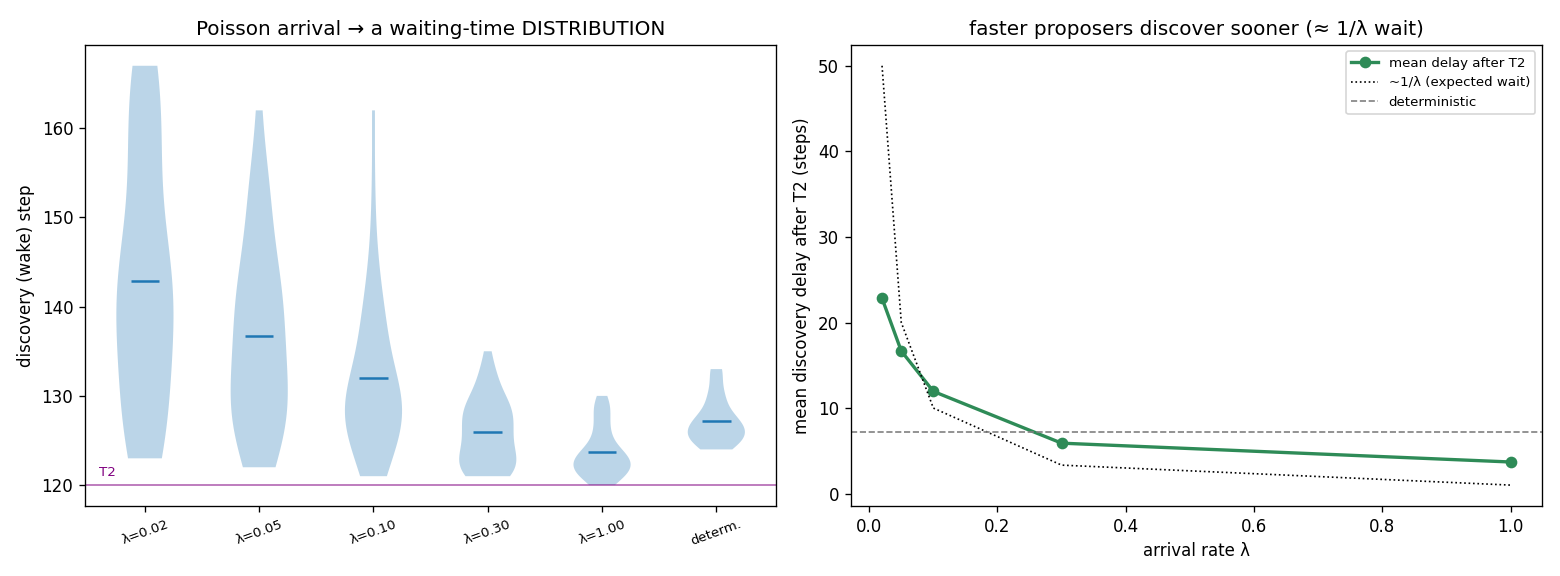
\includegraphics[width=\linewidth]{fig_poisson.png}\caption{exploration as a Poisson rate}
\label{sub:poisson}
\end{subfigure}\hfill
\begin{subfigure}{0.48\textwidth}\centering
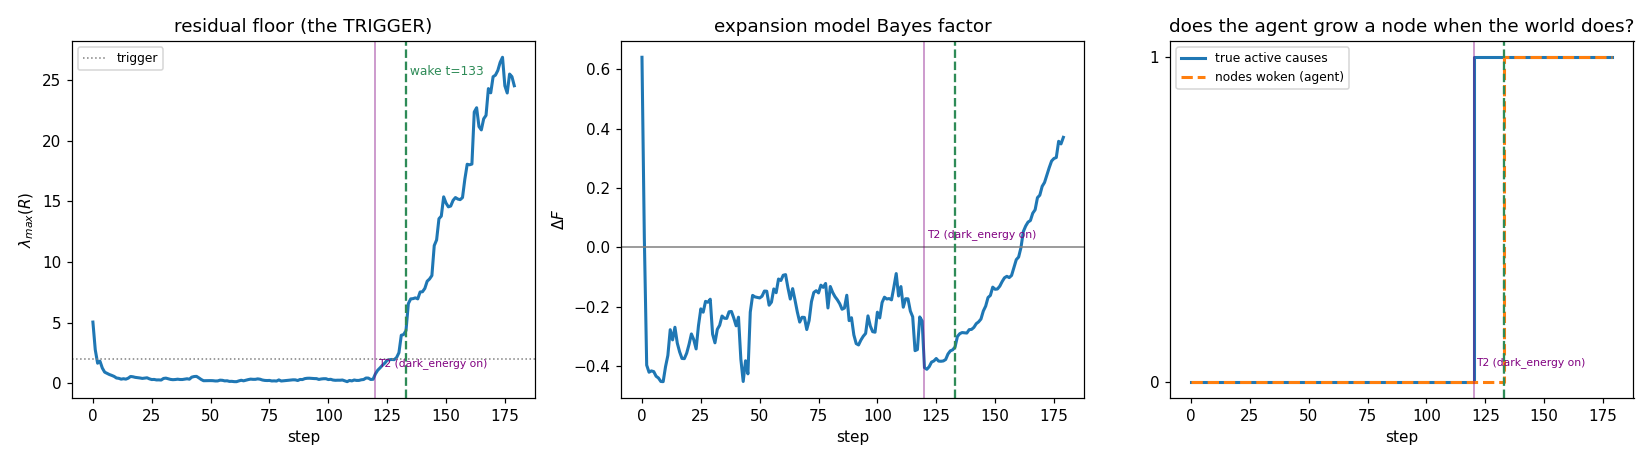
\includegraphics[width=\linewidth]{fig_node_wake.png}\caption{waking an unconceived node}
\label{sub:wake}
\end{subfigure}
\caption{Exploration and expansion. \subref{sub:poisson}~Proposal arrivals as a Poisson process: the
discovery delay after a cause appears is a waiting time of mean $\approx1/\lambda$; at low $\lambda$
some runs never discover the cause within the horizon. \subref{sub:wake}~An agent whose menu lacks
$\Lambda$ wakes a new node \emph{after} the unconceived cause appears at $t=120$ (here $t=133$), never
before; the residual floor (left), the expansion Bayes factor (middle) and the node count (right)
move only once the world makes the missing dimension felt.}
\label{fig:res-explore}
\end{figure}

\subsection{A coarse model resolves a complex world only slowly}
\label{sec:res-coarse}

A last experiment isolates the cost of a coarse Bayes net against a world richer than it. The true
world is a complex twelve-parameter Gaussian with four latent factors (correlated, individually
ambiguous directions); a coarse agent senses only $\mathrm{res}$ random aggregate combinations per
step. Coarser is slower (Fig.~\ref{fig:res-coarse}, left): the time to resolve the world state to
within a fixed tolerance grows from $58$ steps at full resolution to $221$ steps at
$\mathrm{res}=1$, and below a resolution the agent does not finish within the horizon. Adding
forgetting floors the resolution outright (Fig.~\ref{fig:res-coarse}, right): a net that both
under-senses and forgets plateaus at a residual error that rises as $\omega$ falls ($0.08\to0.28$),
and at $\mathrm{res}=3,\,\omega\le0.93$ never resolves the world at all. A complex world has no clear
answer for a bounded, forgetful, under-sensing learner---the honest limit the hidden-structure premise
of \S\ref{sec:hidden} implies.

\begin{figure}[t]
\centering
\begin{subfigure}{0.6\textwidth}\centering
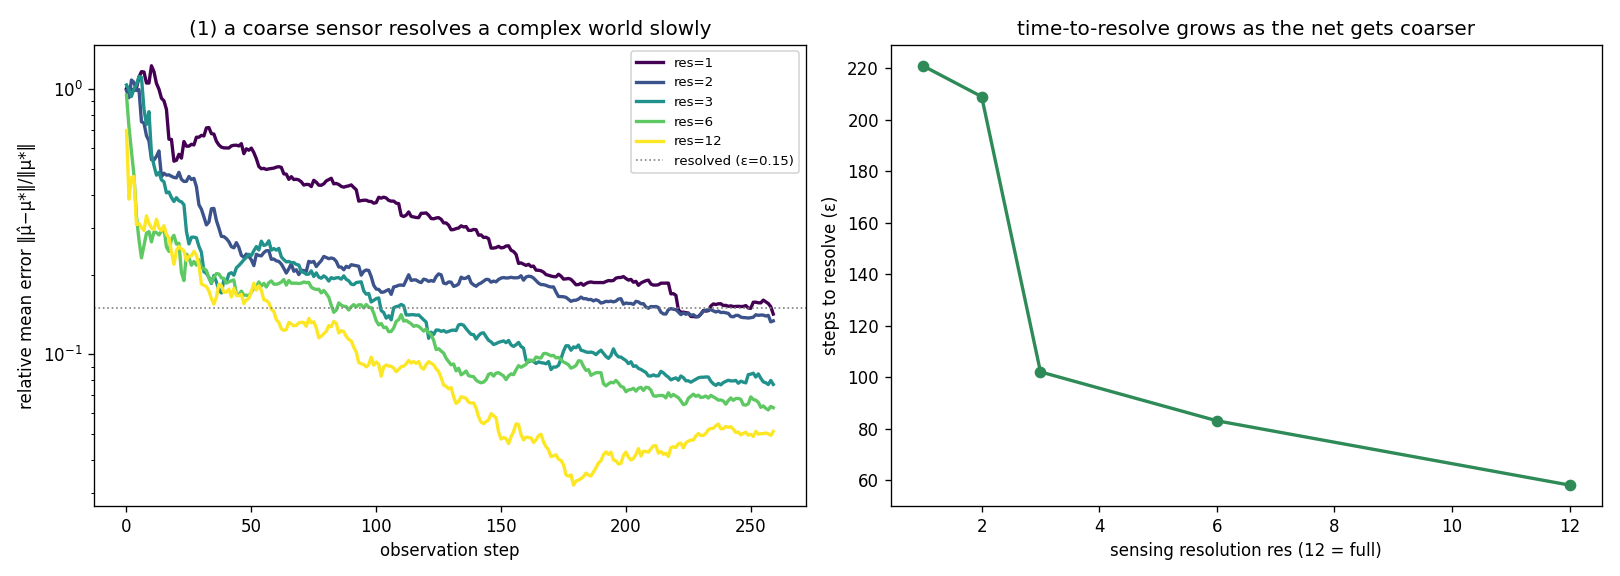
\includegraphics[width=\linewidth]{fig_coarse_resolve.png}\caption{coarser $\Rightarrow$ slower}
\label{sub:coarse}
\end{subfigure}\hfill
\begin{subfigure}{0.38\textwidth}\centering
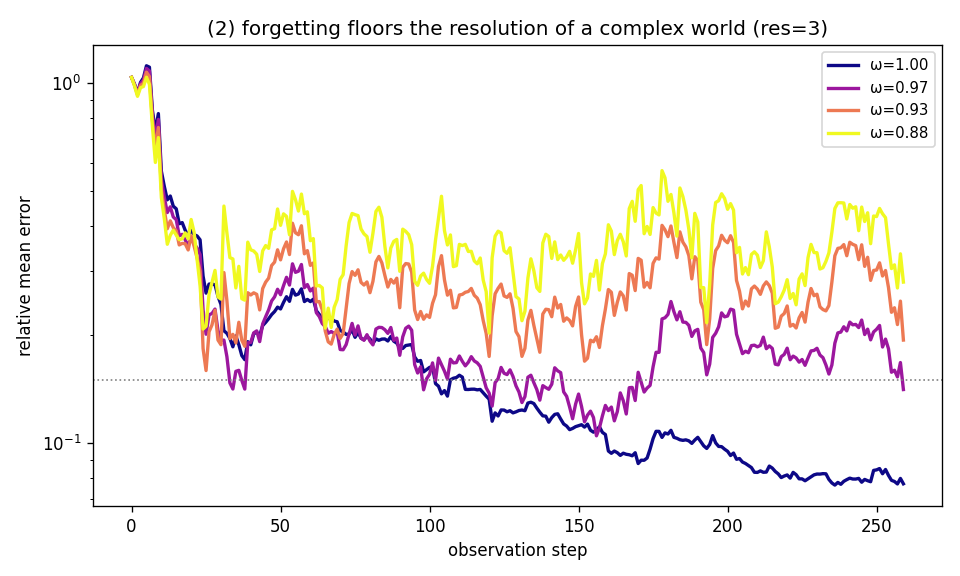
\includegraphics[width=\linewidth]{fig_coarse_floor.png}\caption{forgetting floors it}
\label{sub:floor}
\end{subfigure}
\caption{A coarse net on a complex world. \subref{sub:coarse}~Relative error in the reconstructed
world state over time, by sensing resolution; time-to-resolve grows sharply as the net coarsens.
\subref{sub:floor}~With a fixed coarse sensor, forgetting plateaus the error at a floor that rises as
$\omega$ falls---the world is never fully resolved.}
\label{fig:res-coarse}
\end{figure}

\subsection{Endogenous $\gamma$: lock-in derived from conviction, not imposed}
\label{sec:res-gamma}

The lock-in of \S\ref{sec:res-lockin} was driven by exogenous levers. The paper's sharper claim
(Eqs.~\eqref{eq:gamma}--\eqref{eq:cgf}) is that conviction \emph{itself} silences the channels that
would refute it: a community that values the incumbent drives the disconfirming sensory precisions
$\rho_k$ toward zero, the susceptibility $Z''(\lambda)$ collapses along those directions, and the
core stalls though the evidence is physically present. We make this endogenous. Each round the
observation weight on the disconfirming rows is recomputed as a saturating function of the conviction
field projected onto them, $w_k=\exp(-g\,|U\!\cdot\!H_k|)$, so $\gamma=\overline{1-w_k}$ rises with
the conviction-to-censorship coupling $g$; no channel is gated by hand. On the phlogiston paradigm
(whose disconfirming rows genuinely carry the refuting mass-balance signal) the result is the
$\gamma$-crossover the theory predicts (Fig.~\ref{fig:res-gamma}): as $g$ rises, endogenous $\gamma$
climbs $0\!\to\!1$ and the structural revolution collapses from a revolted fraction of $1.0$ to $0.0$.
The decisive control is \emph{deaf-but-honest}: at the \emph{same} conviction with the gate switched
off, the channels stay open and the community revolts ($1.0$)---so the stall is the conviction-driven
gating, not absent or unreachable evidence. This discharges the caveat that lock-in was merely
lever-imposed: it is derived from $\gamma$ via $Z''(\lambda)\to0$, with honest agents and reachable
truth, exactly the paper's sharpest prediction.

\begin{figure}[t]
\centering
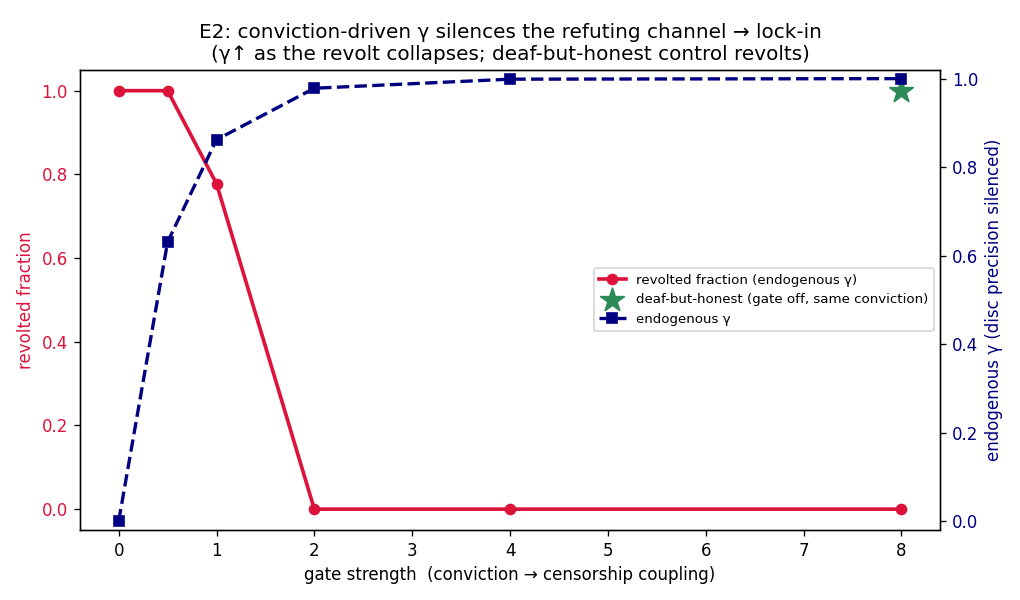
\includegraphics[width=0.6\linewidth]{fig_endogenous_gamma.png}
\caption{Endogenous $\gamma$ (phlogiston). As the conviction-to-censorship coupling $g$ rises, the
conviction field silences its own disconfirming channels: $\gamma$ (navy) climbs to $1$ and the
revolted fraction (crimson) collapses through a sharp crossover---an evidential lock-in
\emph{derived} from conviction. The deaf-but-honest control (green star: same conviction, gate off)
revolts, proving the stall is the gating and not absent evidence.}
\label{fig:res-gamma}
\end{figure}

\subsection{Does a conservatism-gated revision rate recover the staircase? No---and that localizes the gap}
\label{sec:res-staircase}

The other prediction of Fig.~\ref{fig:phase}---a belt-first, core-last staircase in the
conservatism-stratified order parameter---does not appear in the base dynamics because $\kappa$ is a
static read-out that never enters the update. The natural fix is to let $\kappa$ gate the \emph{rate}
of revision: a per-node deposit gate $g_i=1/(1+\beta\kappa_i)$, PD-preserving, so a high-$\kappa$ core
node integrates evidence slower than a cheap belt node. We tested it on phlogiston, and it does
\emph{not} recover the staircase (Fig.~\ref{fig:res-staircase}). The belt$\to$core lag stays negative
($-55$ steps at $\beta=0$, $-45$ at large $\beta$): the high-$\kappa$ nodes reorganize \emph{first},
not last, and the $\kappa$-gradient gate is indistinguishable from a gradient-free uniform slowdown
($-45$) and a shuffled-$\kappa$ gate ($-45$). Two reasons, and they unify this section's two negatives
into one. First, a deposit gate scales both numerator and denominator of the mean $\mu=\Pi^{-1}h$, so
it barely throttles mean-tracking---and mean-tracking is where theory identity lives. Second, the
nodes that actually reorganize are exactly the high-$\kappa$ mass-law commitments the relational
operator refutes directly, while the low-$\kappa$ belt are agreement nodes with nothing to
reorganize, so the conservatism stratification is confounded with move-versus-don't-move. Both reasons
are one root cause: with an operator-set Fisher deposit $J=H^\top H/\sigma^2$---set by the observation
operator, not the data---the structure does not move, so theory identity rides the posterior
\emph{means} and neither a rate gate on those means nor the stratified couplings can express the
staircase. The conservatism gradient $\kappa$ is real and realised statically
(\S\ref{sec:res-twofield}); the negative tells us precisely what is missing to make it temporal: a
\emph{data-dependent} observation model in which the couplings themselves are learned (a
structure-matched or nonlinear operator). That is the central modelling target the result identifies.

\begin{figure}[t]
\centering
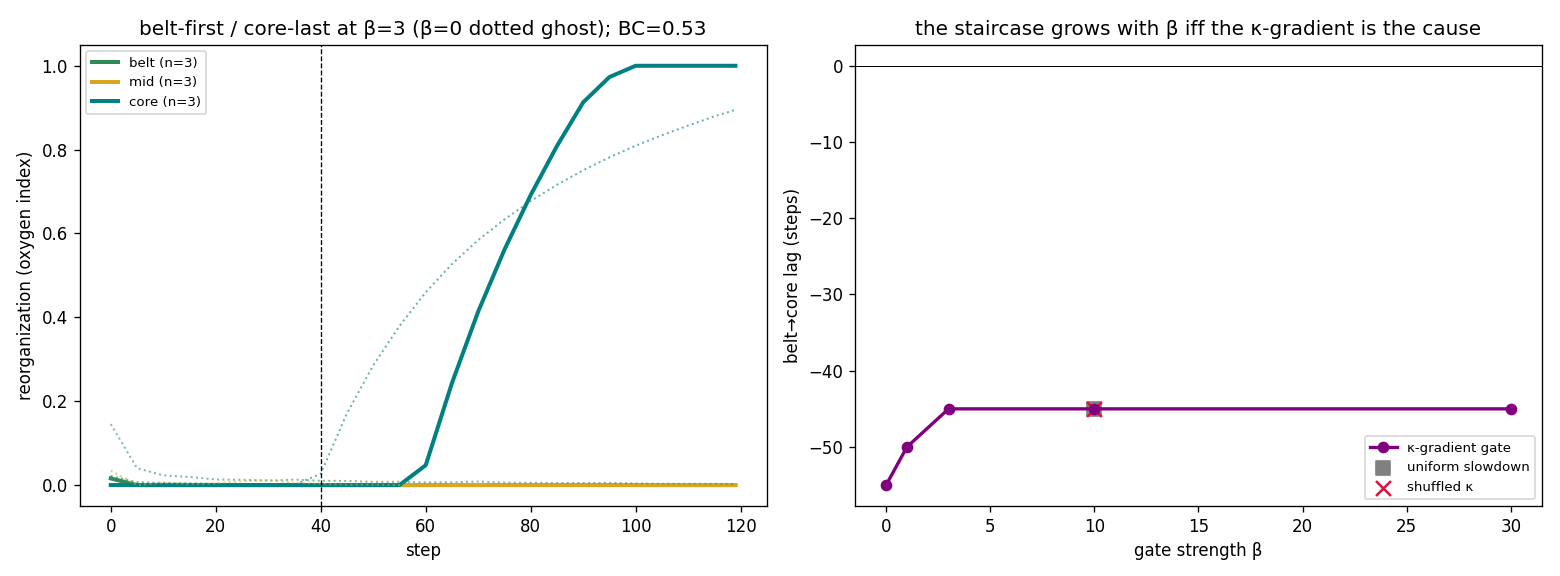
\includegraphics[width=\linewidth]{fig_staircase.png}
\caption{The staircase is \emph{not} recovered by a conservatism-gated revision rate (phlogiston).
\emph{Left:} reorganization by $\kappa$-shell at the best $\beta$ ($\beta=0$ baseline dotted)---the
high-$\kappa$ ``core'' moves first and the low-$\kappa$ ``belt'' (agreement nodes) never reorganizes,
the reverse of the prediction. \emph{Right:} the belt$\to$core lag stays negative and the
$\kappa$-gradient gate (purple) is matched by the gradient-free uniform (grey square) and
shuffled-$\kappa$ (red cross) nulls---the gradient adds nothing. The negative localizes the missing
ingredient to data-dependent structure learning.}
\label{fig:res-staircase}
\end{figure}

\subsection{What remains stylized}
\label{sec:res-caveats}

Two of the section's caveats are now discharged or sharpened: lock-in is \emph{derived} from $\gamma$
(\S\ref{sec:res-gamma}), and the staircase's absence is \emph{localized} to the operator-set Fisher
deposit (\S\ref{sec:res-staircase}). One general caveat stands.

\emph{It is a stylized model.} The dark-energy net is illustrative, its weights chosen to expose the
geometry rather than to fit data; the three dials ($\omega$, $\lambda$, sensing resolution) are swept,
not inferred; and a community that ``tracks'' the eventually-true theory is committed to it, not
thereby correct. Nothing here is evidence about cosmology---it is a model of how a structured,
bounded, valued mind changes.

% ======================================================================
\section{Relation to prior work}
\label{sec:related}
% ======================================================================

The differentiator from the network-epistemology and reinforcement-learning literatures is not the
tool but the explanatory claim, and it is exactly the two debts of Section~\ref{sec:background} now
discharged. Where those models \emph{posit} an exploration bonus and a switching cost, we
\emph{derive} exploration as the epistemic drive to expand the model (realised as a Poisson rate in
\S\ref{sec:res-explore}) and the cost of switching as the carry-over of a structural edit,
$\kappa=\Top\bone$ (realised in \S\ref{sec:res-twofield}). Where those models fix the hypothesis
space, we make it the object of inference---and \S\ref{sec:res-explore} shows the menu itself growing
a node. Much of the accumulated literature recovers as a special case of the one mechanism. The
Zollman speed--accuracy trade-off is the statement of how the algebraic connectivity of the trust
graph governs the transient---denser graphs reorganize faster but lose the transient structural
diversity that protects against locking onto the worse paradigm, exactly the disconnection lever of
\S\ref{sec:res-lockin}; swept directly on the cosmology task, raising $\lambda_2$ drives the
population's residual structural diversity from $3.3$ to $0.2$, and sharing whole posteriors
(conclusions) rather than raw Fisher (evidence) herds it the same way ($3.3\!\to\!0.5$)---the
content-versus-conduit reading of why sharing conclusions propagates bias. The paradoxical finding that confirmation bias can improve group learning is
the same fact read at the agent level, high-$\kappa_i$ agents preserving diversity, with evidential
lock-in as its pathological limit. The bubble-versus-chamber distinction \citep{nguyen2018} is the
formal separation between the sparsity of trust channels and the precision they carry. And Thagard's
connectionist model of explanatory coherence \citep{thagard1989} is recognizable as the
precision-weighted network $p(x\mid G)$ with the gains flattened and the dynamics frozen---a paradigm
net without the active sampling that makes our account move.

% ======================================================================
\section{Discussion}
\label{sec:discussion}
% ======================================================================

The scalar treatment with which the field began is the degenerate single-node limit recovered when the
paradigm has no internal structure, hence no channels to turn down. Everything distinctive follows from
taking the hidden structure seriously: a conservatism gradient derived rather than assigned (one
operator on the unit source), an exploration drive that is the value of expanding the model rather than
a tuned bonus, a cost of change that is the literal re-reading of dependent commitments, a second field
of conviction that is the same operator on a different source and decouples cleanly from conservatism on
the same graph, and a population signature---graded reorganization, or its stall into lock-in---distinct
from a damped oscillation to consensus. Running the model bears the qualitative predictions out: the
two fields come apart on a real net (Fig.~\ref{fig:res-twofield}), lock-in is a genuine and structured
phenomenon requiring conviction and disconnection together (Fig.~\ref{fig:res-tracking}), forgetting
both restores re-tracking and converts lock-in from automatic into earned (Fig.~\ref{fig:res-forgetting}),
and expansion discovers a dimension the menu lacked (Fig.~\ref{fig:res-explore}). It also tells us
precisely where the idealisation must be repaired---the operator-set Fisher deposit that flattens the
staircase (\S\ref{sec:res-staircase})---which is more useful than a clean confirmation would have been.

The Kuhnian reading is now a corollary. Normal science is exploitation: reduction and value-fitting
within a fixed cube of hypotheses. Revolution is exploration: the costly expansion that adds a dimension
the cube did not contain. Incommensurability is the off-diagonal residue of a Schur complement, the
carry-over edge one paradigm's structure deposits when read through another's---the very banana of
Fig.~\ref{fig:res-schur}. And lock-in is the collective amputation of a correction channel.

This also locates what remains genuinely uncertain in a way that resists being made Bayesian, and it is
the point on which the paper opened. Structure learning navigates beautifully within the dimensions a
model posits, but it is blind to the dimension no one has proposed---the node not yet drawn even as a
dashed candidate. That frontier is the Knightian residue, and it is precisely Stanford's problem of
unconceived alternatives \citep{stanford2006}: not uncertainty over which known structure is right,
which the precision cube renders measurable, but uncertainty over whether the space of known structures
contains the truth at all. A community doing only reduction is in permanent normal science; the
unmeasurable possibility that the whole cube is misspecified is what expansion, and only expansion, can
resolve. One cannot place a posterior over the unconceived; running an expansion process that keeps
proposing nodes---at some Poisson rate---is what a healthy epistemic system does instead of pretending it
can, and \S\ref{sec:res-explore} shows both that it works and that too low a rate leaves the dimension
undiscovered. The hidden structure of the world, which forced us into structure learning on the first
page, is in the end the thing no amount of structure learning can guarantee to have caught---and it is on
that frontier that the curator's external hand on $\pi_s$ becomes most consequential, able to push a
population across the lock-in boundary from the outside by ensuring that the revisions which would expand
the cube are never sampled.

% ======================================================================
\begin{thebibliography}{99}\small

\bibitem[Albarracin et al.(2022)]{albarracin2022}
M.~Albarracin, D.~Demekas, M.~J.~D.~Ramstead, and C.~Heins.
Epistemic communities under active inference. \emph{Entropy}, 24(4):476, 2022.

\bibitem[Dalege et al.(2016)]{dalege2016}
J.~Dalege, D.~Borsboom, F.~van Harreveld, H.~van den Berg, M.~Conner, and H.~L.~J.~van der Maas.
Toward a formalized account of attitudes: the Causal Attitude Network (CAN) model.
\emph{Psychological Review}, 123(1):2--22, 2016.

\bibitem[Friedman et al.(2008)]{friedman2008glasso}
J.~Friedman, T.~Hastie, and R.~Tibshirani.
Sparse inverse covariance estimation with the graphical lasso.
\emph{Biostatistics}, 9(3):432--441, 2008.

\bibitem[Friston and Penny(2011)]{friston2011}
K.~J.~Friston and W.~Penny.
Post hoc Bayesian model selection. \emph{NeuroImage}, 56(4):2089--2099, 2011.

\bibitem[Friston et al.(2015)]{friston2015}
K.~Friston, F.~Rigoli, D.~Ognibene, C.~Mathys, T.~Fitzgerald, and G.~Pezzulo.
Active inference and epistemic value. \emph{Cognitive Neuroscience}, 6(4):187--214, 2015.

\bibitem[Friston et al.(2017)]{friston2017curiosity}
K.~J.~Friston, M.~Lin, C.~D.~Frith, G.~Pezzulo, J.~A.~Hobson, and S.~Ondobaka.
Active inference, curiosity and insight. \emph{Neural Computation}, 29(10):2633--2683, 2017.

\bibitem[Friston et al.(2018)]{friston2018bmr}
K.~J.~Friston, T.~Parr, and P.~Zeidman.
Bayesian model reduction. arXiv:1805.07092, 2018.

\bibitem[Hyland and Albarracin(2025)]{hyland2025}
D.~Hyland and M.~Albarracin.
On the variational costs of changing our minds. arXiv:2509.17957, 2025.
(Also in \emph{Active Inference: IWAI 2025}, CCIS vol.~2857, Springer, 2026,
doi:10.1007/978-3-032-16955-6\_1.)

\bibitem[Jonard et al.(2025)]{jonard2025}
N.~Jonard et al.
Theory choice in epistemic networks: five ways to avoid premature convergence. PhilSci Archive, 2025.

\bibitem[Kitcher(1990)]{kitcher1990}
P.~Kitcher.
The division of cognitive labor. \emph{Journal of Philosophy}, 87(1):5--22, 1990.

\bibitem[Koller and Friedman(2009)]{koller2009}
D.~Koller and N.~Friedman.
\emph{Probabilistic Graphical Models: Principles and Techniques}. MIT Press, 2009.

\bibitem[Kuhn(1962)]{kuhn1962}
T.~S.~Kuhn.
\emph{The Structure of Scientific Revolutions}. University of Chicago Press, 1962.

\bibitem[MacKay(1992)]{mackay1992}
D.~J.~C.~MacKay.
Bayesian interpolation. \emph{Neural Computation}, 4(3):415--447, 1992.

\bibitem[Millidge et al.(2021)]{millidge2021}
B.~Millidge, A.~Tschantz, and C.~L.~Buckley.
Whence the expected free energy? \emph{Neural Computation}, 33(2):447--482, 2021.

\bibitem[Neal(1996)]{neal1996}
R.~M.~Neal.
\emph{Bayesian Learning for Neural Networks}.
Lecture Notes in Statistics 118, Springer, 1996.

\bibitem[Nguyen(2018)]{nguyen2018}
C.~T.~Nguyen.
Echo chambers and epistemic bubbles. \emph{Episteme}, 17(2):141--161, 2018.

\bibitem[O'Connor and Weatherall(2019)]{oconnor2019}
C.~O'Connor and J.~O.~Weatherall.
\emph{The Misinformation Age}. Yale University Press, 2019.

\bibitem[Smith et al.(2020)]{smith2020structure}
R.~Smith, P.~Schwartenbeck, T.~Parr, and K.~J.~Friston.
An active inference approach to modeling structure learning: concept learning as an example case.
\emph{Frontiers in Computational Neuroscience}, 14:41, 2020.

\bibitem[Stanford(2006)]{stanford2006}
P.~K.~Stanford.
\emph{Exceeding Our Grasp: Science, History, and the Problem of Unconceived Alternatives}.
Oxford University Press, 2006.

\bibitem[Strevens(2003)]{strevens2003}
M.~Strevens.
The role of the priority rule in science. \emph{Journal of Philosophy}, 100(2):55--79, 2003.

\bibitem[Thagard(1989)]{thagard1989}
P.~Thagard.
Explanatory coherence. \emph{Behavioral and Brain Sciences}, 12(3):435--467, 1989.

\bibitem[Tipping(2001)]{tipping2001}
M.~E.~Tipping.
Sparse Bayesian learning and the relevance vector machine.
\emph{Journal of Machine Learning Research}, 1:211--244, 2001.

\bibitem[Zollman(2010)]{zollman2010}
K.~J.~S.~Zollman.
The epistemic benefit of transient diversity. \emph{Erkenntnis}, 72(1):17--35, 2010.

\bibitem[Griffiths and Ghahramani(2011)]{griffiths2011ibp}
T.~L.~Griffiths and Z.~Ghahramani.
The Indian Buffet Process: an introduction and review.
\emph{Journal of Machine Learning Research}, 12:1185--1224, 2011.

\bibitem[Kemp and Tenenbaum(2008)]{kemp2008form}
C.~Kemp and J.~B.~Tenenbaum.
The discovery of structural form.
\emph{Proceedings of the National Academy of Sciences}, 105(31):10687--10692, 2008.

\bibitem[Ullman et al.(2012)]{ullman2012}
T.~D.~Ullman, N.~D.~Goodman, and J.~B.~Tenenbaum.
Theory learning as stochastic search in a language of thought.
\emph{Cognitive Development}, 27(4):455--480, 2012.

\bibitem[Williams and Beer(2010)]{williams2010pid}
P.~L.~Williams and R.~D.~Beer.
Nonnegative decomposition of multivariate information. arXiv:1004.2515, 2010.

\bibitem[Friston et al.(2017b)]{friston2017process}
K.~Friston, T.~FitzGerald, F.~Rigoli, P.~Schwartenbeck, and G.~Pezzulo.
Active inference: a process theory. \emph{Neural Computation}, 29(1):1--49, 2017.

\bibitem[Mathys et al.(2011)]{mathys2011}
C.~Mathys, J.~Daunizeau, K.~J.~Friston, and K.~E.~Stephan.
A Bayesian foundation for individual learning under uncertainty.
\emph{Frontiers in Human Neuroscience}, 5:39, 2011.

\bibitem[Smith et al.(2022)]{smith2022tutorial}
R.~Smith, K.~J.~Friston, and C.~Whyte.
A step-by-step tutorial on active inference and its application to empirical data.
\emph{Journal of Mathematical Psychology}, 107:102632, 2022.

\bibitem[Da Costa et al.(2020)]{dacosta2020}
L.~Da Costa, T.~Parr, N.~Sajid, S.~Veselic, V.~Neacsu, and K.~Friston.
Active inference on discrete state-spaces: a synthesis.
\emph{Journal of Mathematical Psychology}, 99:102447, 2020.

\bibitem[Holmes(2000)]{holmes2000}
F.~L.~Holmes.
The revolution in chemistry and physics: overthrow of a reigning paradigm or competition between
contemporary research programs? \emph{Isis}, 91(4):735--753, 2000.

\bibitem[Thagard(1990)]{thagard1990}
P.~Thagard.
The conceptual structure of the chemical revolution.
\emph{Philosophy of Science}, 57(2):183--209, 1990.

\bibitem[Boantza and Gal(2011)]{boantza2011}
V.~D.~Boantza and O.~Gal.
The `absolute existence' of phlogiston: the losing party's point of view.
\emph{British Journal for the History of Science}, 44(3):317--342, 2011.

\bibitem[Blumenthal and Ladyman(2017)]{blumenthal2017}
G.~Blumenthal and J.~Ladyman.
The development of problems within the phlogiston theories, 1766--1791.
\emph{Foundations of Chemistry}, 19(3):241--280, 2017.

\bibitem[Ball et al.(2024)]{polygraphs2024}
B.~Ball, A.~Koliousis, A.~Mohanan, and M.~Peacey.
Computational philosophy: reflections on the {PolyGraphs} project.
\emph{Humanities and Social Sciences Communications}, 11:186, 2024.

\bibitem[Michelini et al.(2023)]{michelini2023}
M.~Michelini, J.~Osorio, W.~Houkes, D.~\v{S}e\v{s}elja, and C.~Stra\ss{}er.
Scientific disagreements and the diagnosticity of evidence: how too much data may lead to polarization.
\emph{Journal of Artificial Societies and Social Simulation}, 26(4):5, 2023.

\bibitem[Albarracin et al.(2024)]{albarracin2024protentions}
M.~Albarracin, R.~J.~Pitliya, T.~St.~Clere Smithe, D.~A.~Friedman, K.~Friston, and M.~J.~D.~Ramstead.
Shared protentions in multi-agent active inference.
\emph{Entropy}, 26(4):303, 2024.

\bibitem[Friston et al.(2024a)]{friston2023federated}
K.~J.~Friston, T.~Parr, C.~Heins, A.~Constant, D.~Friedman, T.~Isomura, C.~Fields,
T.~Verbelen, M.~Ramstead, J.~Clippinger, and C.~D.~Frith.
Federated inference and belief sharing.
\emph{Neuroscience \& Biobehavioral Reviews}, 156:105500, 2024.

\bibitem[Waade et al.(2025)]{waade2025}
P.~T.~Waade, C.~L.~Olesen, J.~E.~Laursen, S.~W.~Nehrer, C.~Heins, K.~Friston, and C.~Mathys.
As one and many: relating individual and emergent group-level generative models in active inference.
\emph{Entropy}, 27(2):143, 2025.

\bibitem[Ullman and Tenenbaum(2020)]{ullman2020}
T.~D.~Ullman and J.~B.~Tenenbaum.
Bayesian models of conceptual development: learning as building models of the world.
\emph{Annual Review of Developmental Psychology}, 2:533--558, 2020.

\bibitem[Smith et al.(2022b)]{smith2022plos}
R.~Smith, V.~Neacsu, M.~B.~Mirza, R.~A.~Adams, and K.~J.~Friston.
Simulating empirical phenomena of inference under active learning and active selection through
{Bayesian} model reduction. \emph{PLOS ONE}, 17(12):e0277199, 2022.

\bibitem[Priorelli and Stoianov(2023)]{priorelli2023}
M.~Priorelli and I.~P.~Stoianov.
Dynamic inference by model reduction.
\emph{bioRxiv}, 2023. doi:10.1101/2023.09.10.557043.

\bibitem[Friston et al.(2016)]{friston2016peb}
K.~J.~Friston, V.~Litvak, A.~Oswal, A.~Razi, K.~E.~Stephan, B.~C.~M.~van Wijk, G.~Ziegler, and
P.~Zeidman. Bayesian model reduction and empirical {Bayes} for group ({DCM}) studies.
\emph{NeuroImage}, 128:413--431, 2016.

\bibitem[Friston et al.(2024b)]{friston2024ci}
K.~J.~Friston et al.
Designing ecosystems of intelligence from first principles.
\emph{Collective Intelligence}, 3(4), 2024. arXiv:2212.01354.

\bibitem[Kaufmann et al.(2021)]{kaufmann2021}
R.~Kaufmann, P.~Gupta, and J.~Taylor.
An active inference model of collective intelligence.
\emph{Entropy}, 23(7):830, 2021.

\end{thebibliography}

\end{document}
